\subsection{Lịch sử phát triển của mạng CNN}
Mạng nơ-ron tích chập (Convolutional Neural Network - CNN) là một trong những kiến trúc quan trọng nhất trong lĩnh vực Thị giác máy tính (Computer Vision). CNN được thiết kế nhằm khai thác cấu trúc không gian của dữ liệu ảnh, giúp mô hình tự động học đặc trưng thay vì phải thiết kế thủ công như các phương pháp truyền thống.

Quá trình phát triển của CNN trải qua nhiều giai đoạn quan trọng:

\begin{itemize}
    \item \textbf{Thập niên 1980:} Kunihiko Fukushima giới thiệu mô hình \textbf{Neocognitron}, lấy cảm hứng từ hệ thần kinh thị giác sinh học.
    \item \textbf{Năm 1998:} Yann LeCun phát triển \textbf{LeNet-5}, mạng CNN đầu tiên đạt thành công thực tiễn trong nhận dạng chữ số viết tay.
    \item \textbf{Năm 2012:} Mạng \textbf{AlexNet} chiến thắng cuộc thi ImageNet với sai số vượt trội, mở ra kỷ nguyên Deep Learning.
    \item \textbf{Năm 2015:} \textbf{ResNet} sử dụng Residual Learning và Skip Connection, giải quyết vấn đề mất gradient khi huấn luyện mạng rất sâu.
\end{itemize}

\subsection{Kiến trúc và nguyên lý hoạt động của CNN}
Một kiến trúc CNN điển hình bao gồm các thành phần: Lớp tích chập (Convolution Layer), Lớp kích hoạt (Activation Function), Lớp gộp (Pooling Layer) và các Lớp kết nối đầy đủ (Fully Connected Layers).

\subsubsection{Lớp Tích chập (Convolution Layer)}
Lớp Convolution là trái tim của CNN, thực hiện phép tích chập giữa bộ lọc (kernel/filter) và vùng ảnh đầu vào. Công thức toán học:

\begin{equation}
    (f * g)(i,j) = \sum_{m} \sum_{n} f(m,n) \cdot g(i-m, j-n)
\end{equation}

\textbf{Các siêu tham số quan trọng:}
\begin{itemize}
    \item \textbf{Kích thước kernel:} Thường là 3×3 hoặc 5×5, ảnh hưởng đến receptive field.
    \item \textbf{Số lượng kernel:} Xác định số feature maps đầu ra.
    \item \textbf{Stride:} Bước nhảy của kernel, ảnh hưởng đến kích thước output.
    \item \textbf{Padding:} Thêm viền để giữ nguyên kích thước (same padding) hoặc giảm (valid padding).
\end{itemize}

\subsubsection{Lớp Kích hoạt (Activation Functions)}
Hàm kích hoạt giới thiệu tính phi tuyến vào mạng, cho phép học các pattern phức tạp:
\begin{itemize}
    \item \textbf{ReLU (Rectified Linear Unit):} $f(x) = max(0, x)$ - Giải quyết vanishing gradient, phổ biến nhất.
    \item \textbf{Sigmoid:} $f(x) = \frac{1}{1+e^{-x}}$ - Đưa về [0,1], phù hợp cho binary classification.
    \item \textbf{Tanh:} $f(x) = \frac{e^x - e^{-x}}{e^x + e^{-x}}$ - Đưa về [-1,1], zero-centered.
    \item \textbf{Softmax:} $f(x_i) = \frac{e^{x_i}}{\sum_j e^{x_j}}$ - Cho multi-class classification.
\end{itemize}

\subsubsection{Lớp Gộp (Pooling Layer)}
Pooling giảm kích thước feature map, tăng tính bất biến không gian và giảm tham số:
\begin{itemize}
    \item \textbf{Max Pooling:} Lấy giá trị lớn nhất trong vùng, giữ lại đặc trưng mạnh nhất.
    \item \textbf{Average Pooling:} Lấy trung bình, làm mịn feature map.
    \item \textbf{Global Average Pooling:} Trung bình toàn bộ feature map, thay thế FC layers.
\end{itemize}

\subsubsection{Lớp Kết nối Đầy đủ (Fully Connected Layer)}
FC layers thực hiện classification dựa trên features đã trích xuất. Tuy nhiên, chúng có nhiều tham số và dễ overfitting.

\subsubsection{Các Kiến trúc CNN Hiện đại}
\begin{itemize}
    \item \textbf{VGGNet:} Sử dụng kernel 3×3 nhỏ, stack nhiều layers.
    \item \textbf{ResNet:} Skip connections giải quyết degradation problem.
    \item \textbf{Inception:} Multiple kernel sizes trong cùng layer.
    \item \textbf{MobileNet:} Depthwise separable convolution cho mobile devices.
\end{itemize}

\subsubsection{Huấn luyện CNN}
\begin{itemize}
    \item \textbf{Hàm mất mát:} Cross-entropy cho classification, MSE cho regression.
    \item \textbf{Optimizer:} Adam, SGD với momentum, RMSprop.
    \item \textbf{Regularization:} Dropout, Batch Normalization, Data Augmentation.
    \item \textbf{Transfer Learning:} Fine-tuning pretrained models.
\end{itemize}

\subsection{Thực nghiệm theo từng dataset}

Trong phần này, chúng ta sẽ thực hiện xây dựng và huấn luyện các mô hình CNN trên hai bộ dữ liệu tiêu chuẩn: MNIST và Fashion-MNIST. Quy trình bao gồm từ EDA (Exploratory Data Analysis) đến thiết kế kiến trúc mạng và đánh giá kết quả.

Trước tiên, chúng ta thiết lập môi trường lập trình với TensorFlow và Keras.

\begin{figure}[H]
    \centering
    
\includegraphics[width=0.9\textwidth]{../code/ch2_cnn/images/1.png}
    \caption{Khởi tạo các thư viện Deep Learning và cấu hình môi trường đồ họa Seaborn cho các biểu đồ phân tích.}
\end{figure}

\textbf{Giải thích chi tiết:} Đoạn code này thiết lập stack công nghệ cho deep learning. TensorFlow 2.x với Keras API cung cấp high-level interface cho việc xây dựng mạng neural. Numpy xử lý tensor operations, matplotlib/seaborn tạo visualizations. Cấu hình 'Agg' backend tránh xung đột GUI trên headless servers. Việc import theo chuẩn đảm bảo reproducibility và compatibility giữa các phiên bản thư viện.

\subsubsection{Bài toán 1: Nhận dạng chữ số viết tay với MNIST}
MNIST là bộ dữ liệu cơ bản nhưng cực kỳ quan trọng để kiểm tra khả năng trích xuất đặc trưng không gian của lớp Convolution.

\begin{figure}[H]
    \centering
    
\includegraphics[width=0.9\textwidth]{../code/ch2_cnn/images/2.png}
    \caption{Nạp dữ liệu MNIST và thực hiện chuẩn hóa pixel về khoảng [0, 1] để tăng tốc độ hội tụ của Gradient Descent.}
\end{figure}

\textbf{Giải thích chi tiết:} MNIST loader của Keras tự động download và cache dataset. Reshape (60000, 28, 28, 1) chuẩn bị cho CNN input. Normalization x/255.0 đưa pixel từ [0,255] về [0,1], giúp gradient descent hội tụ nhanh hơn vì weights initialization thường quanh 0. Việc này cũng tránh vanishing/exploding gradients và làm cho learning rate dễ tune hơn.

\begin{figure}[H]
    \centering
    
\includegraphics[width=0.9\textwidth]{../code/ch2_cnn/images/3.png}
    \caption{Mã nguồn thực hiện trực quan hóa dữ liệu MNIST, bao gồm mẫu ảnh, phân phối lớp và cường độ điểm ảnh.}
\end{figure}

\textbf{Giải thích chi tiết:} EDA code sử dụng matplotlib để plot sample images, class distribution histogram, và pixel intensity distribution. Việc kiểm tra balance của classes quan trọng vì imbalance có thể bias model. Pixel distribution cho thấy hầu hết pixels là 0 (background), giúp hiểu sparsity của data và lựa chọn activation functions phù hợp.

Dưới đây là các phân tích trực quan thu được từ bước EDA trên bộ MNIST:

\begin{figure}[H]
    \centering
    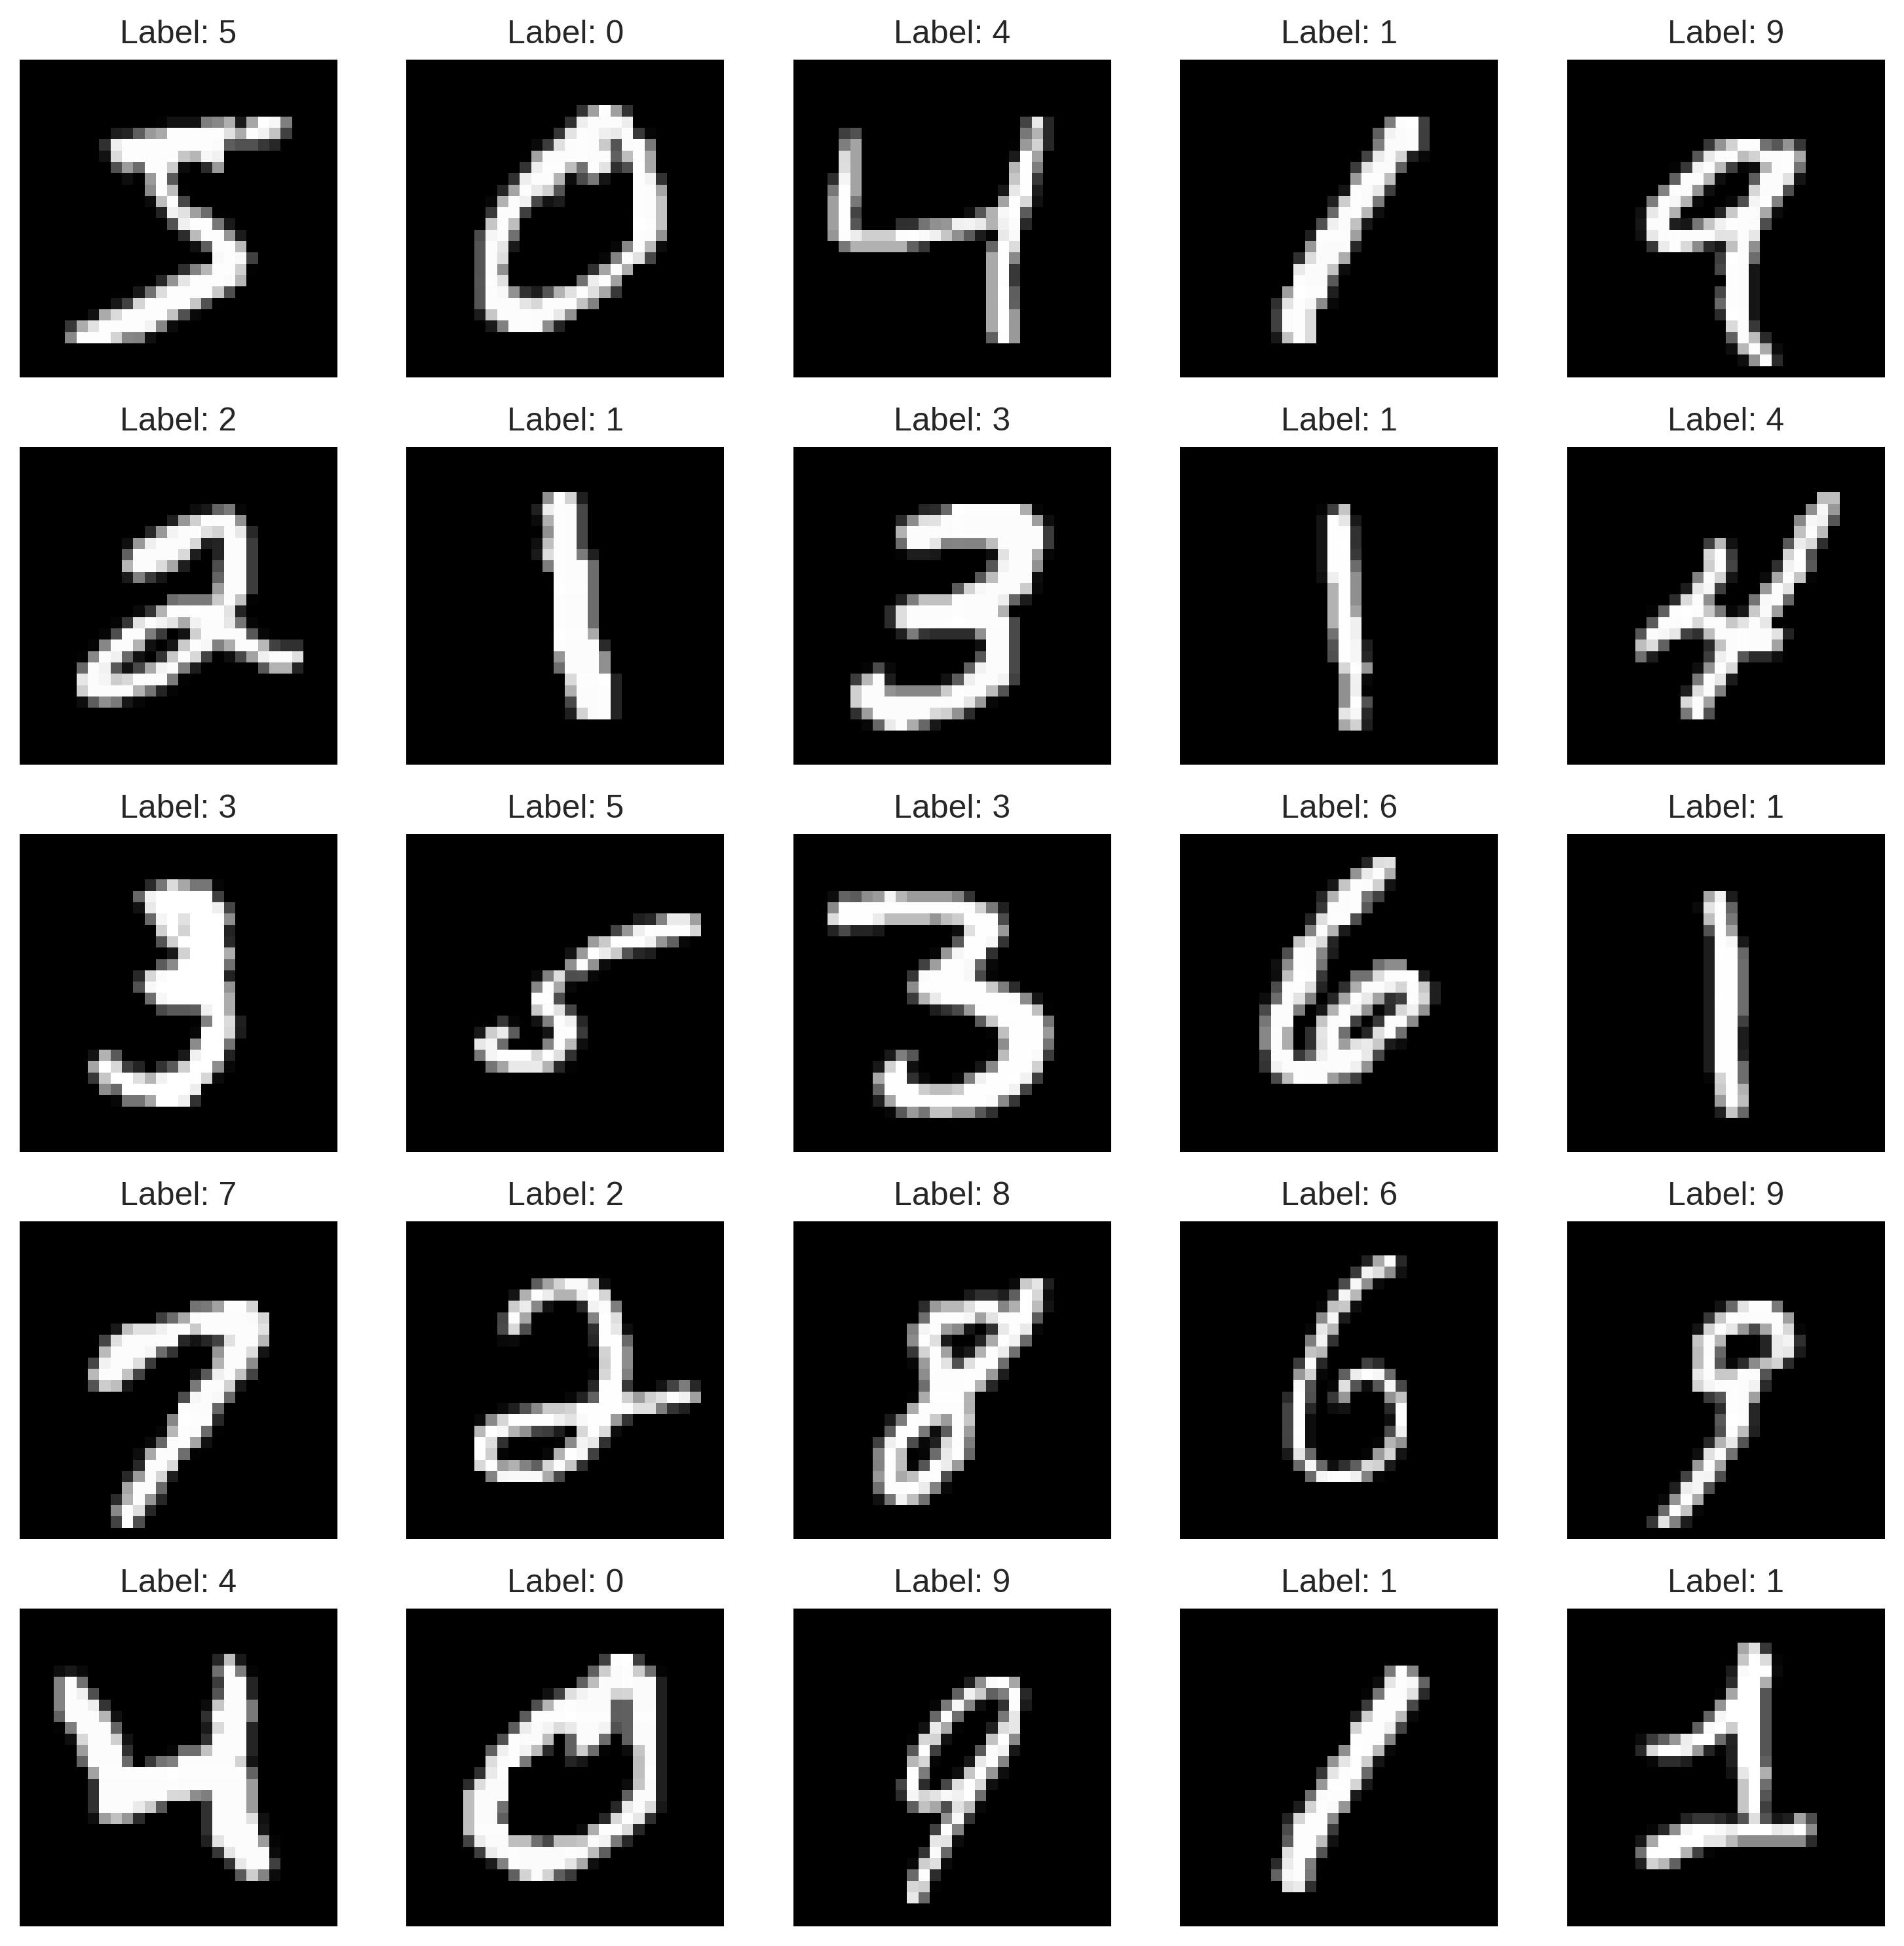
\includegraphics[width=0.75\textwidth]{../code/ch2_cnn/plots/mnist_sample_images.png}
    \caption{Mẫu ảnh MNIST: Trực quan hóa 25 mẫu ảnh ngẫu nhiên cùng nhãn tương ứng, xác nhận dữ liệu đã được nạp đúng định dạng.}
\end{figure}

\begin{figure}[H]
    \centering
    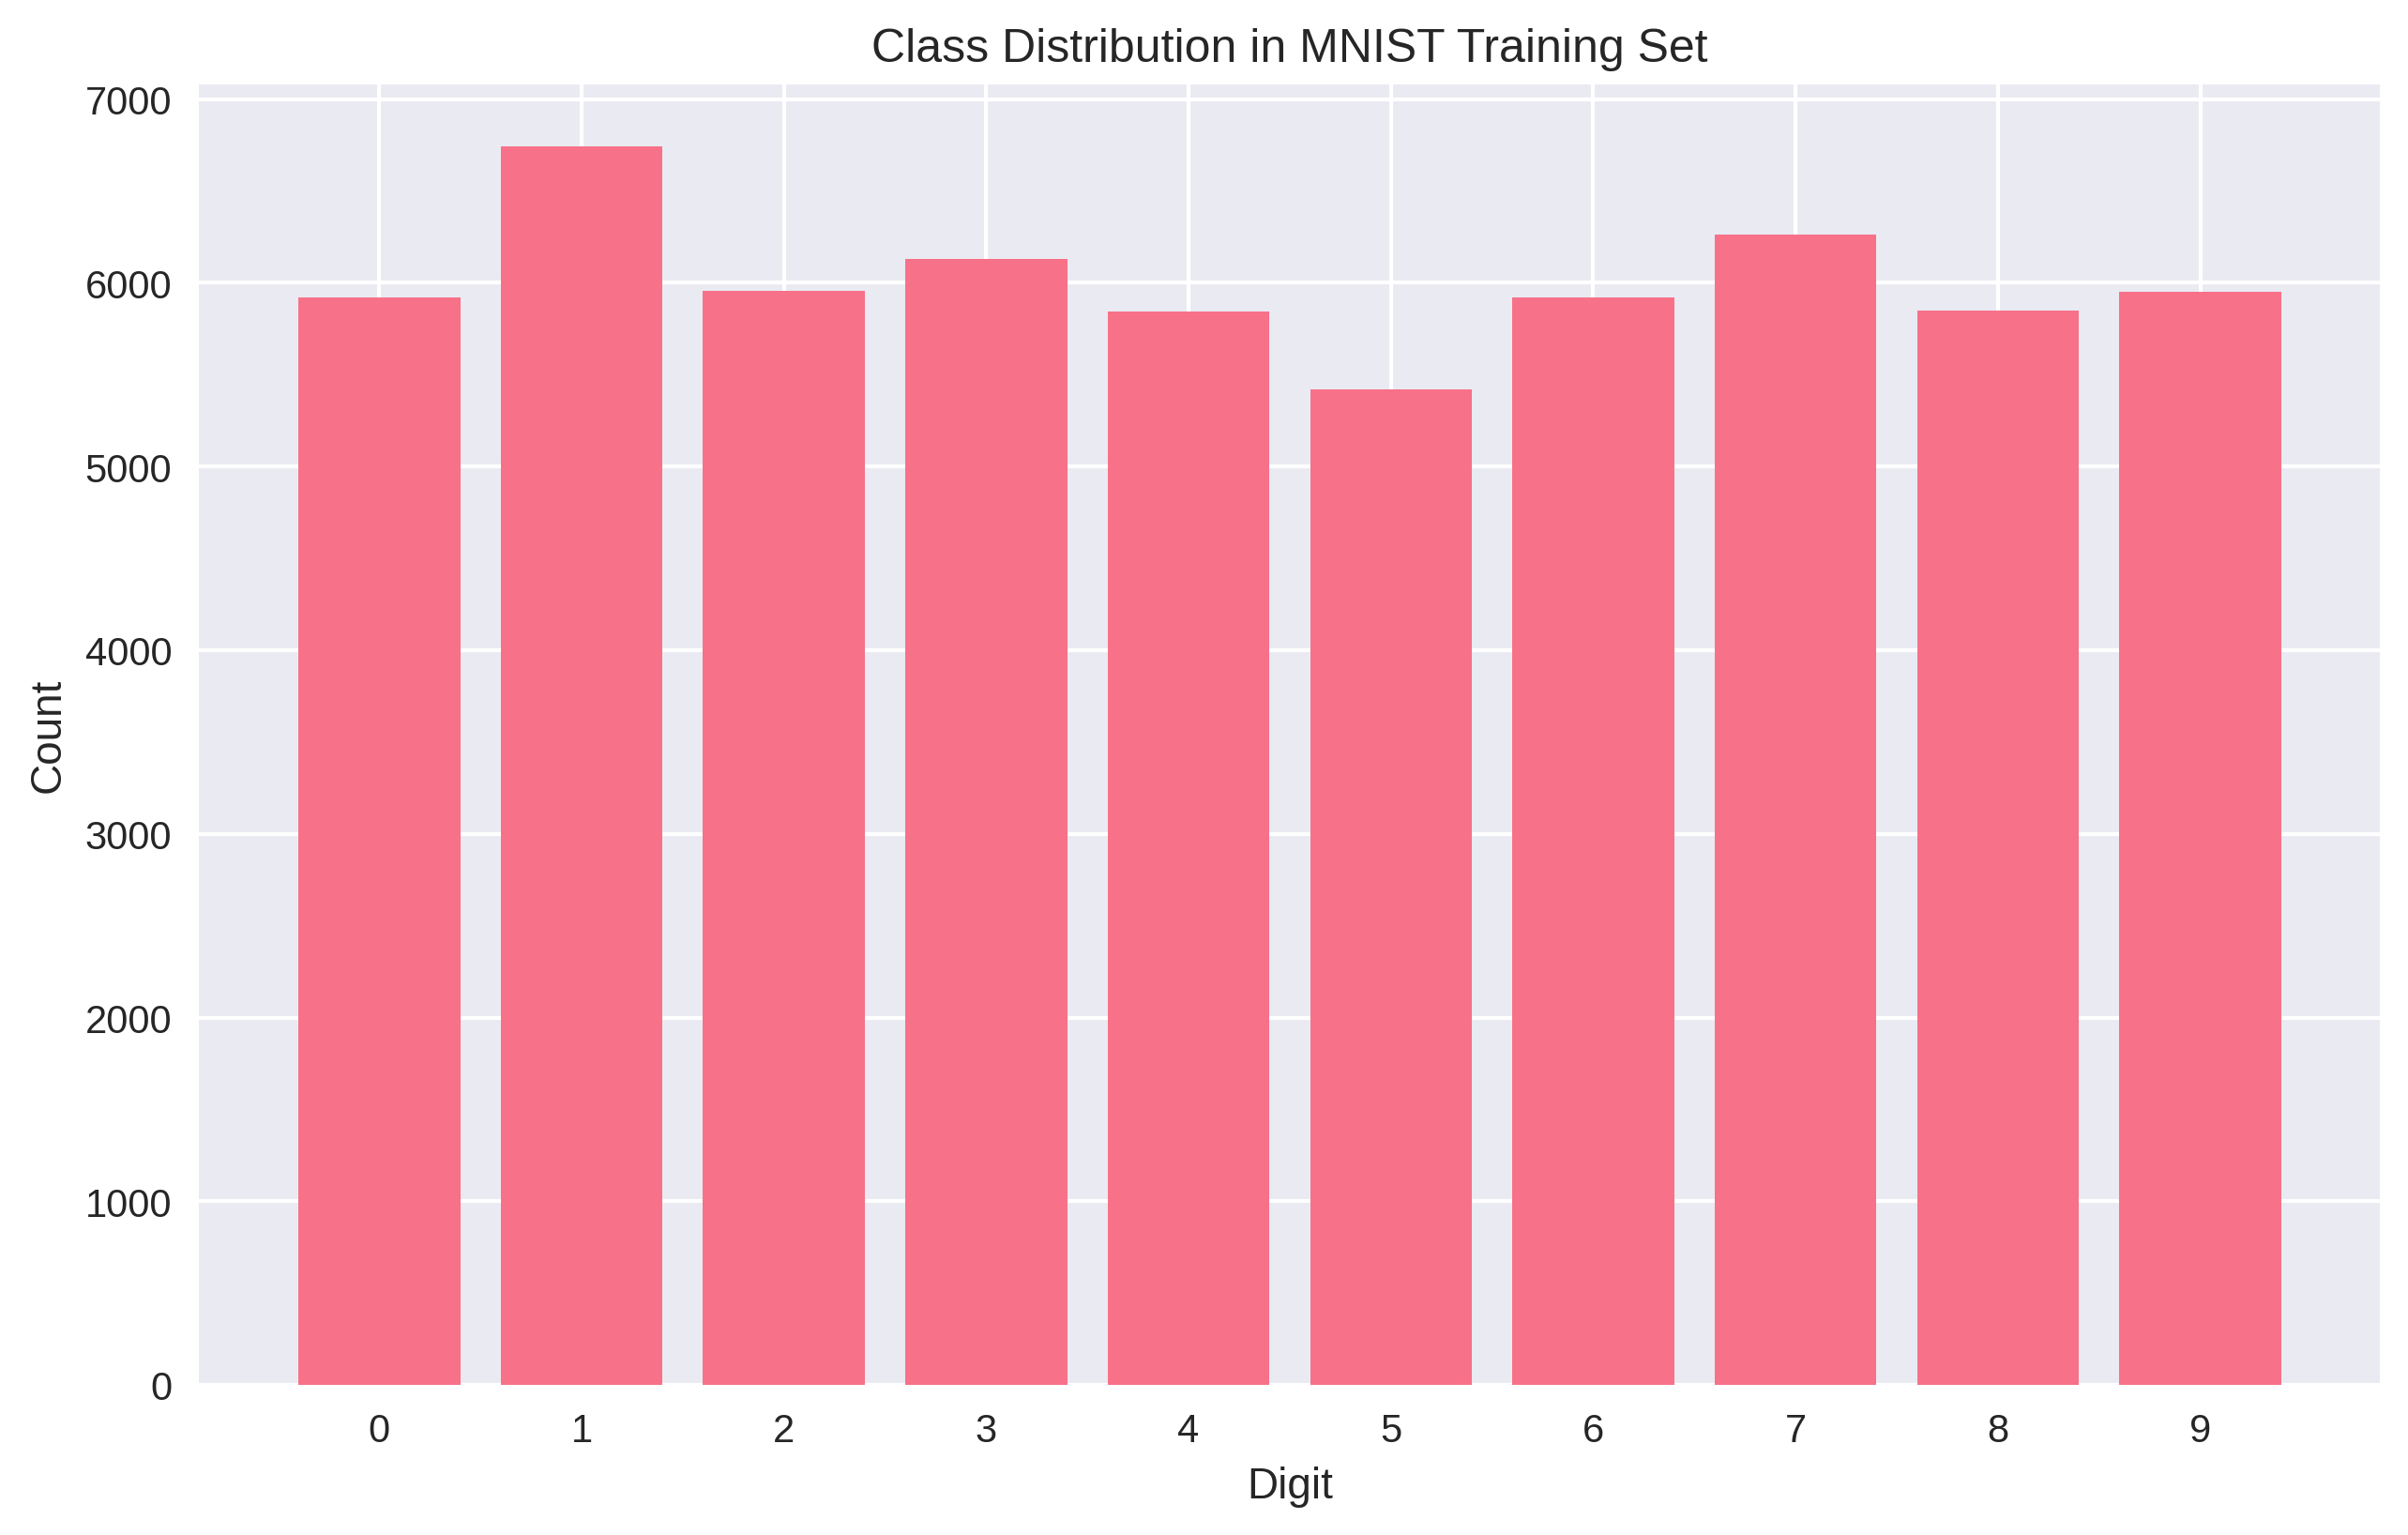
\includegraphics[width=0.75\textwidth]{../code/ch2_cnn/plots/mnist_class_distribution.png}
    \caption{Phân phối lớp: Biểu đồ cột cho thấy sự cân bằng tuyệt vời giữa 10 chữ số, giúp mô hình tránh được hiện tượng thiên lệch (bias).}
\end{figure}

\begin{figure}[H]
    \centering
    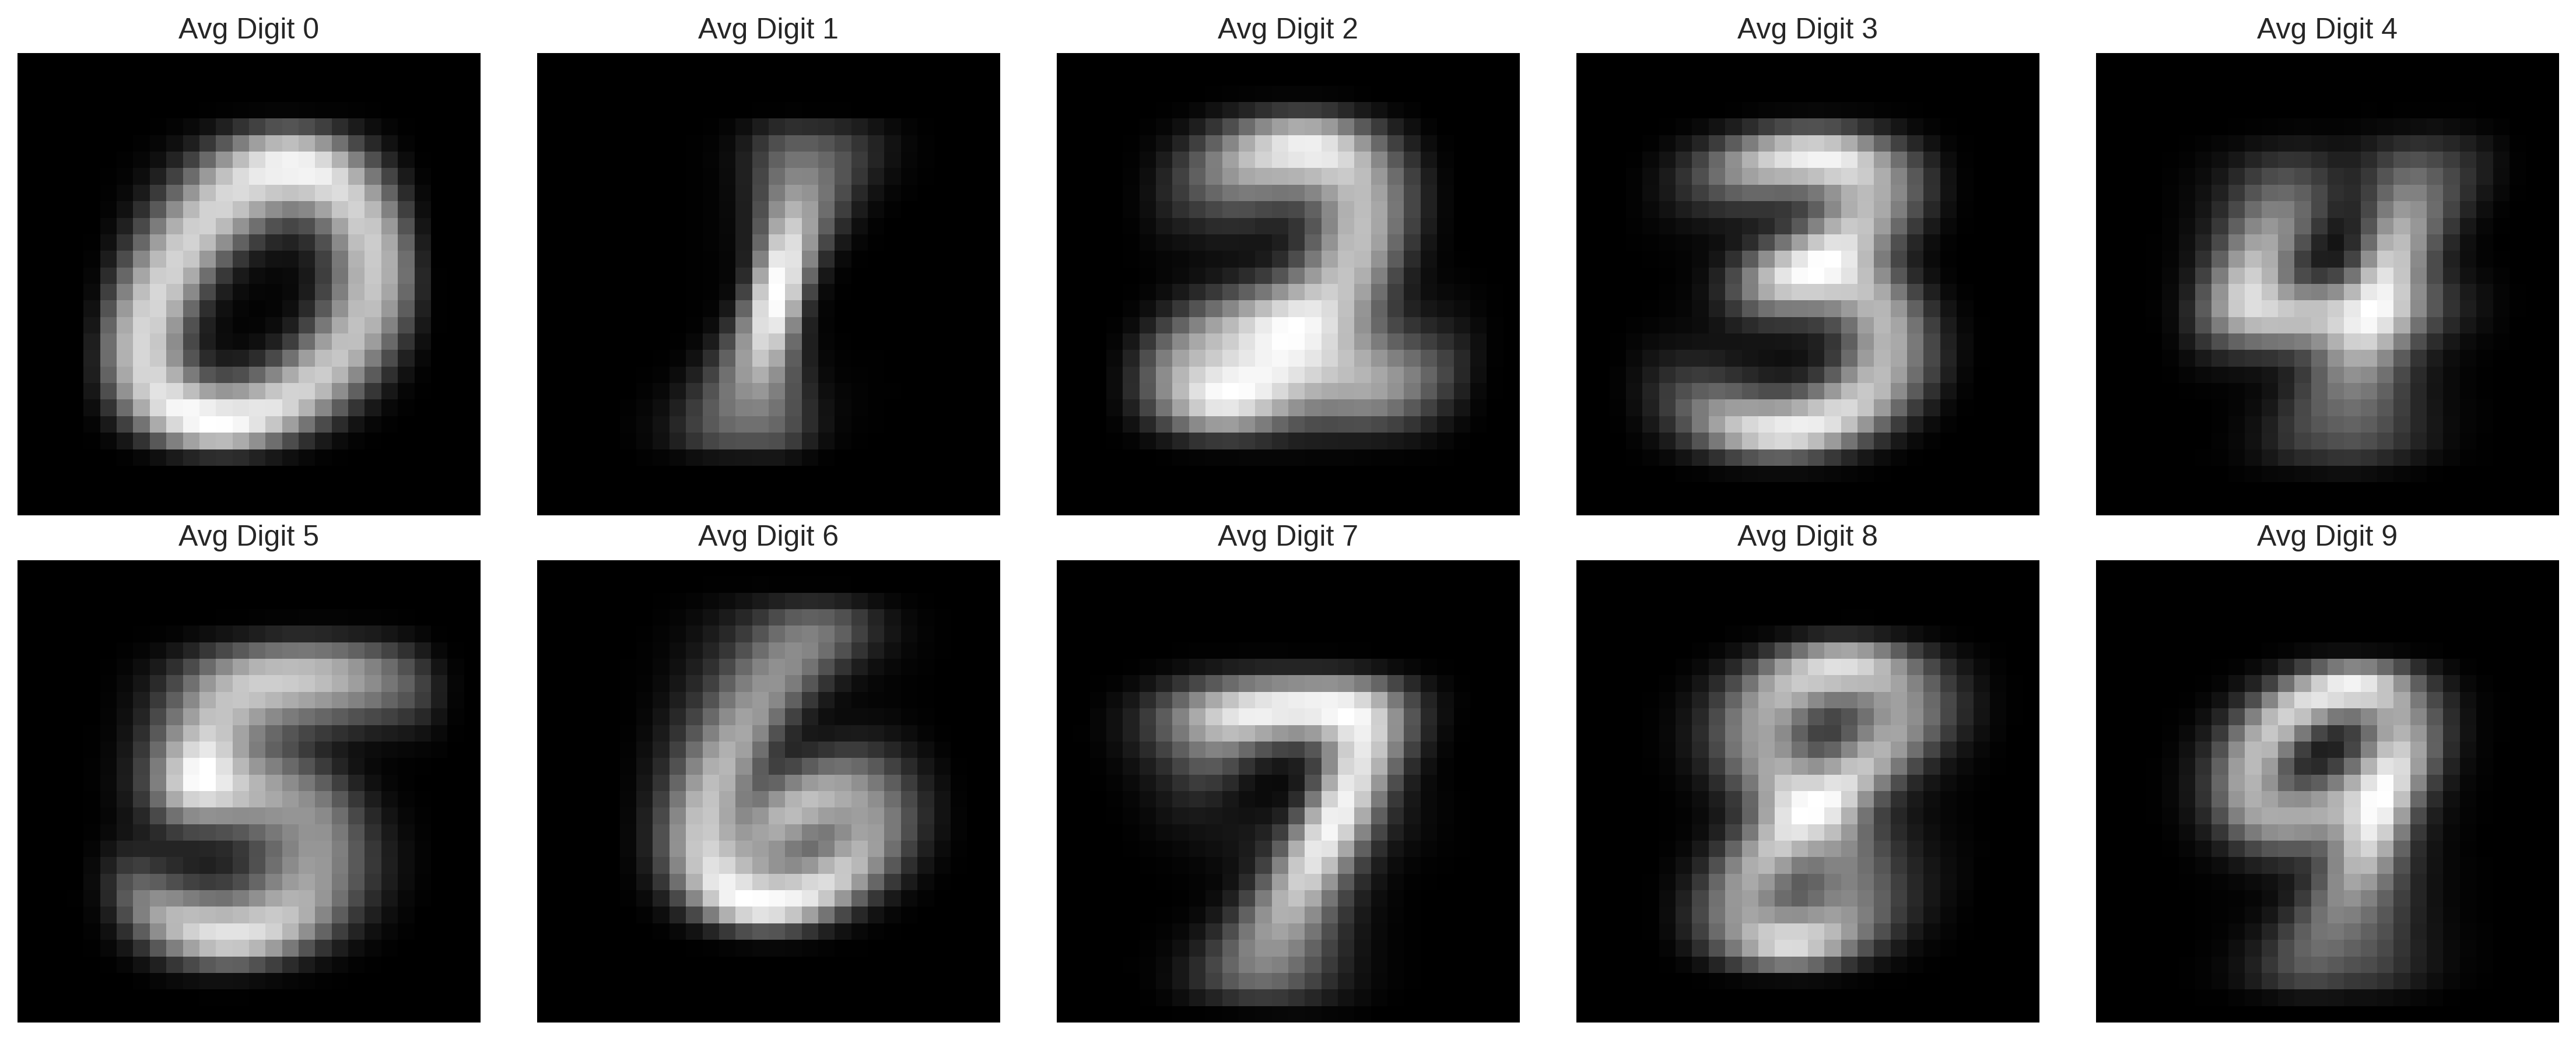
\includegraphics[width=0.75\textwidth]{../code/ch2_cnn/plots/mnist_average_digits.png}
    \caption{Ảnh trung bình theo lớp: Thể hiện hình dạng lý tưởng của mỗi chữ số sau khi lấy trung bình hàng nghìn mẫu, làm nổi bật đặc trưng hình học cốt lõi.}
\end{figure}

\begin{figure}[H]
    \centering
    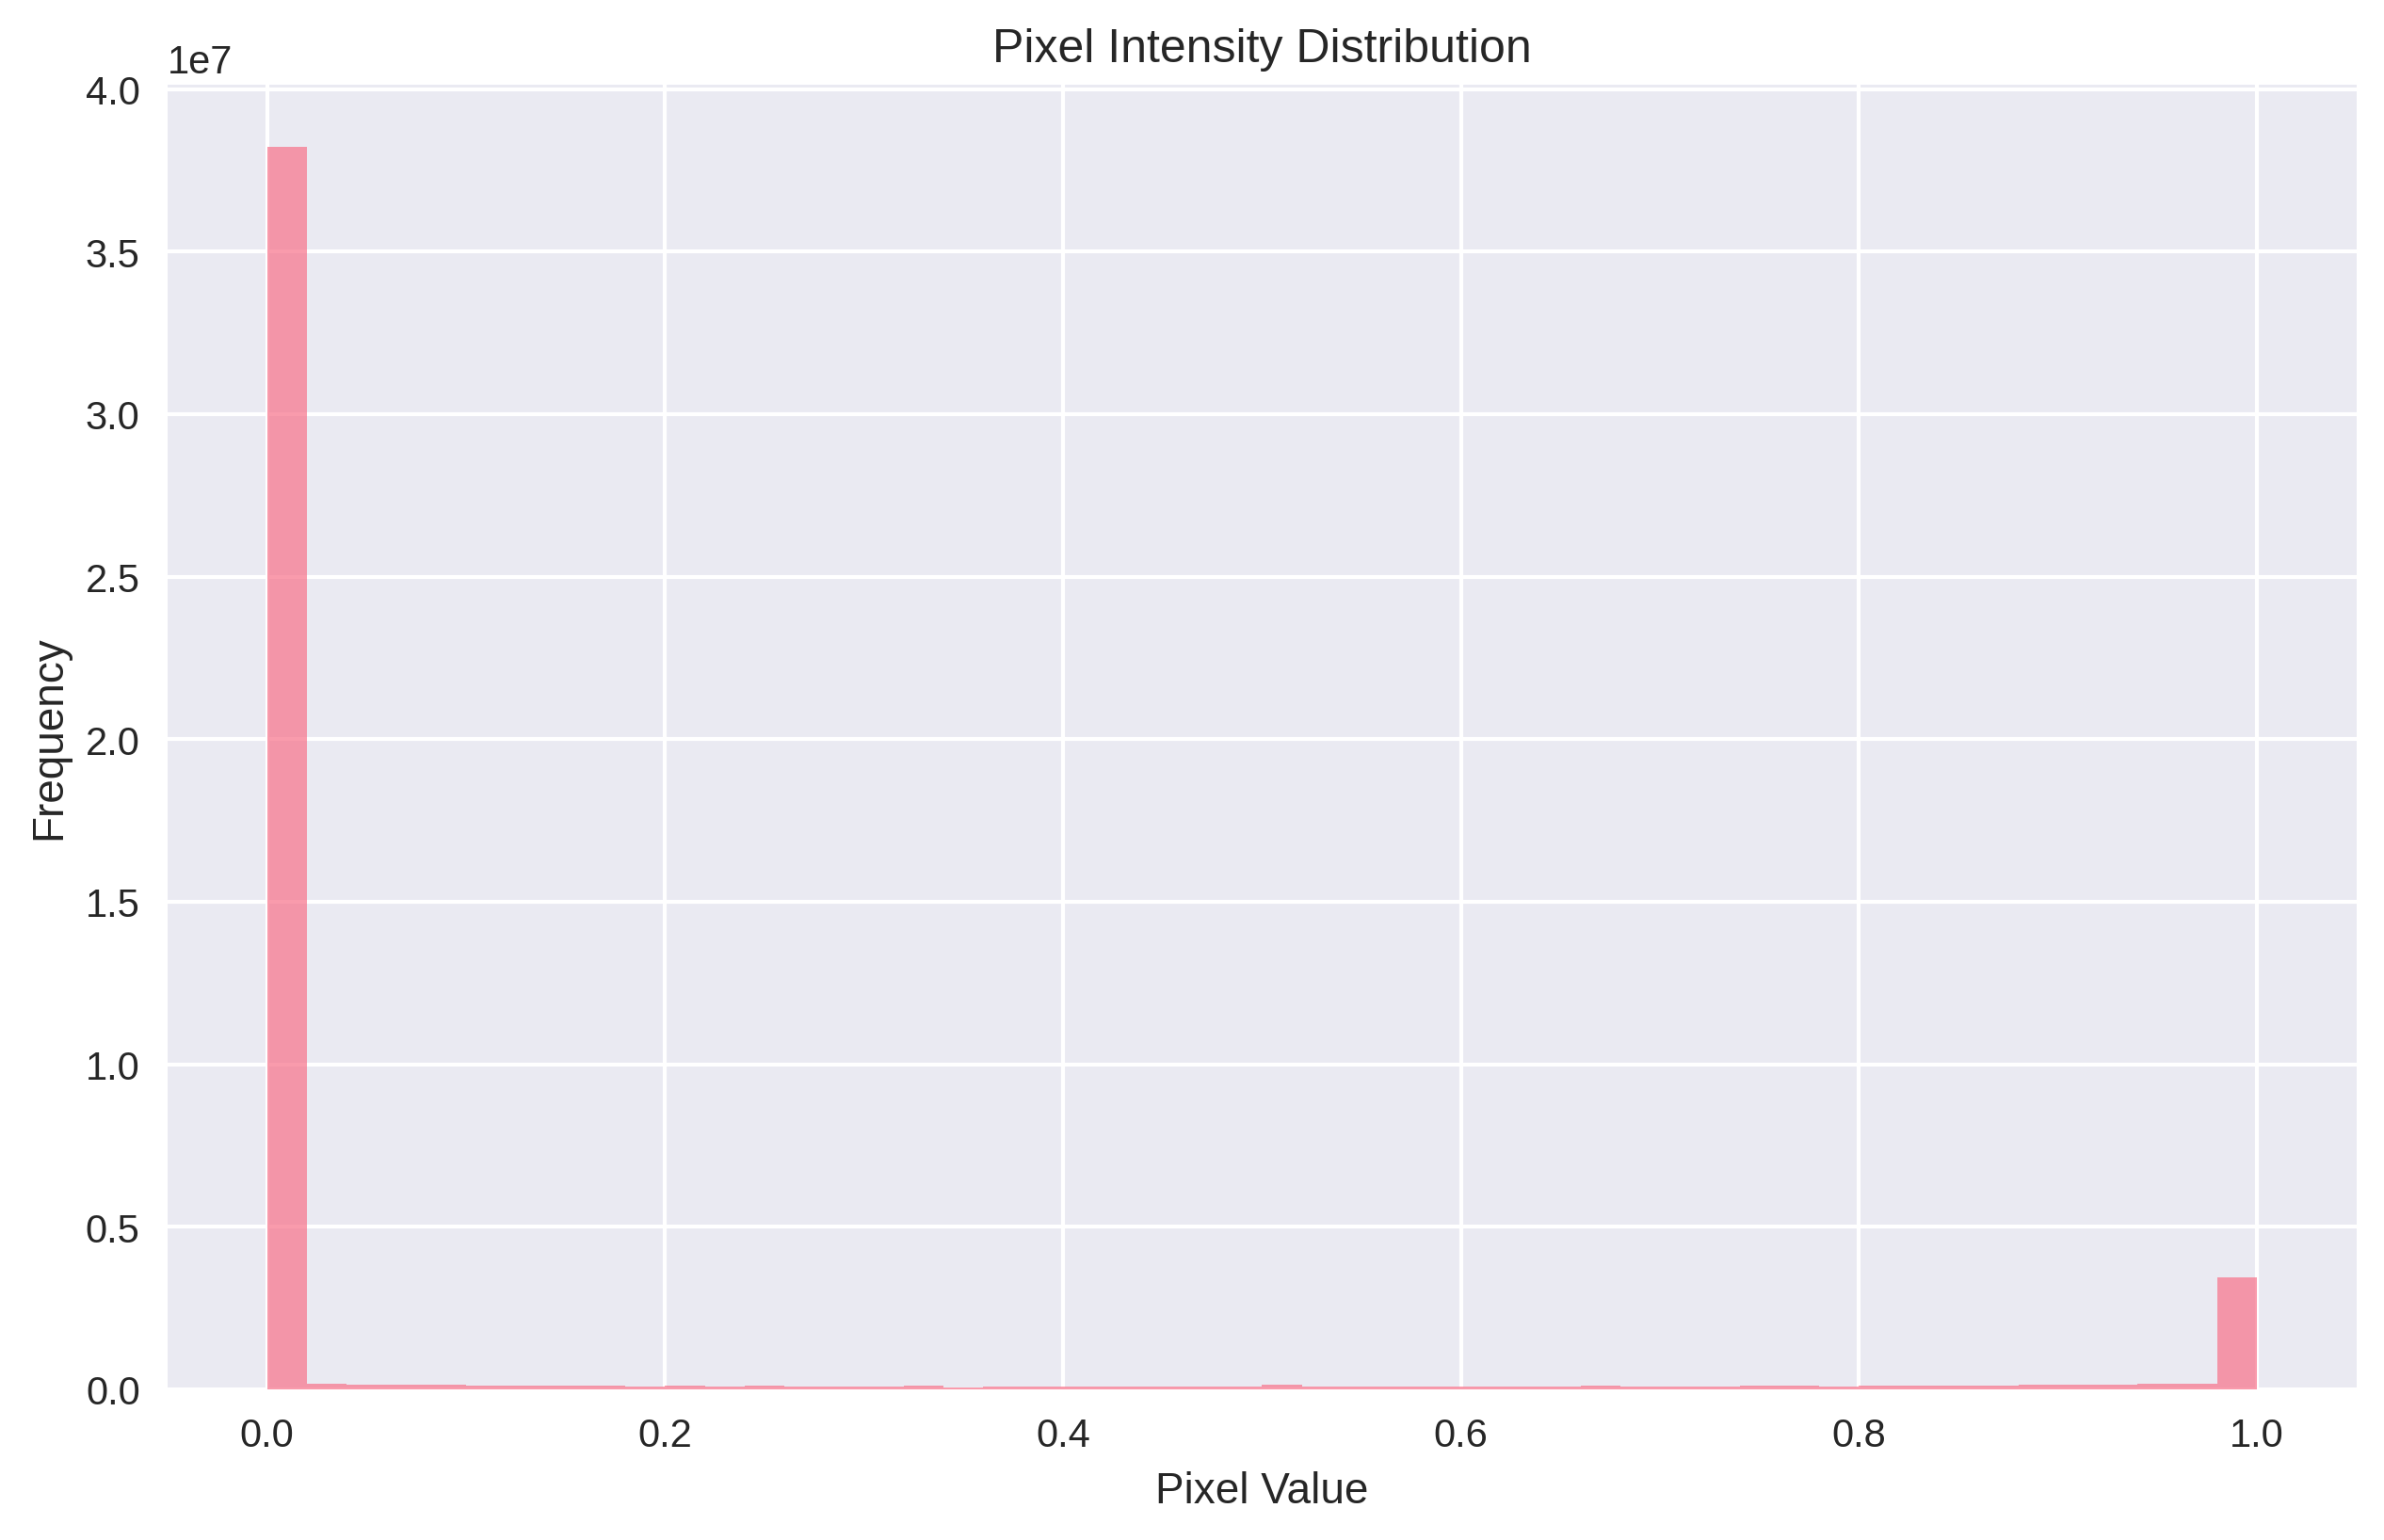
\includegraphics[width=0.75\textwidth]{../code/ch2_cnn/plots/mnist_pixel_intensity_distribution.png}
    \caption{Phân phối cường độ Pixel: Cho thấy hầu hết các điểm ảnh có giá trị gần 0 (nền đen) hoặc gần 1 (nét vẽ), phản ánh tính thưa (sparsity) của dữ liệu.}
\end{figure}

Tiếp theo, chúng ta định nghĩa và xây dựng mô hình CNN.

\begin{figure}[H]
    \centering
    
\includegraphics[width=0.9\textwidth]{../code/ch2_cnn/images/4.png}
    \caption{Thiết kế kiến trúc Simple CNN: Sử dụng các lớp Conv2D để trích xuất đặc trưng và MaxPooling để giảm kích thước bản đồ đặc trưng.}
\end{figure}

\textbf{Phân tích kiến trúc:} Lớp \texttt{Conv2D} thực hiện phép tính tích chập giữa ảnh đầu vào và các bộ lọc (kernels). Mỗi bộ lọc sẽ học cách nhận diện một đặc trưng cụ thể (ví dụ: nét ngang, nét dọc). Lớp \texttt{MaxPooling} đi kèm đóng vai trò quan trọng trong việc tạo ra tính "bất biến dịch chuyển" (Translation Invariance), giúp mô hình vẫn nhận ra chữ số ngay cả khi nó bị lệch nhẹ trong khung hình.

\begin{figure}[H]
    \centering
    
\includegraphics[width=0.9\textwidth]{../code/ch2_cnn/images/5.png}
    \caption{Tóm tắt kiến trúc mạng (Model Summary): Hiển thị số lượng tham số huấn luyện tại mỗi lớp, giúp quản lý độ phức tạp của mô hình.}
\end{figure}

Tiến hành huấn luyện mô hình Simple CNN và so sánh với kiến trúc LeNet-5 cổ điển.

\begin{figure}[H]
    \centering
    
\includegraphics[width=0.9\textwidth]{../code/ch2_cnn/images/6.png}
    \caption{Quá trình huấn luyện Simple CNN trên 5 epochs, theo dõi độ chính xác (Accuracy) và hàm mất mát (Loss).}
\end{figure}

\begin{figure}[H]
    \centering
    
\includegraphics[width=0.9\textwidth]{../code/ch2_cnn/images/7.png}
    \caption{Triển khai mạng LeNet-5: Sử dụng hàm kích hoạt Tanh và lớp AveragePooling theo đúng kiến trúc nguyên bản của Yann LeCun.}
\end{figure}

Kết quả đánh giá mô hình MNIST:

\begin{figure}[H]
    \centering
    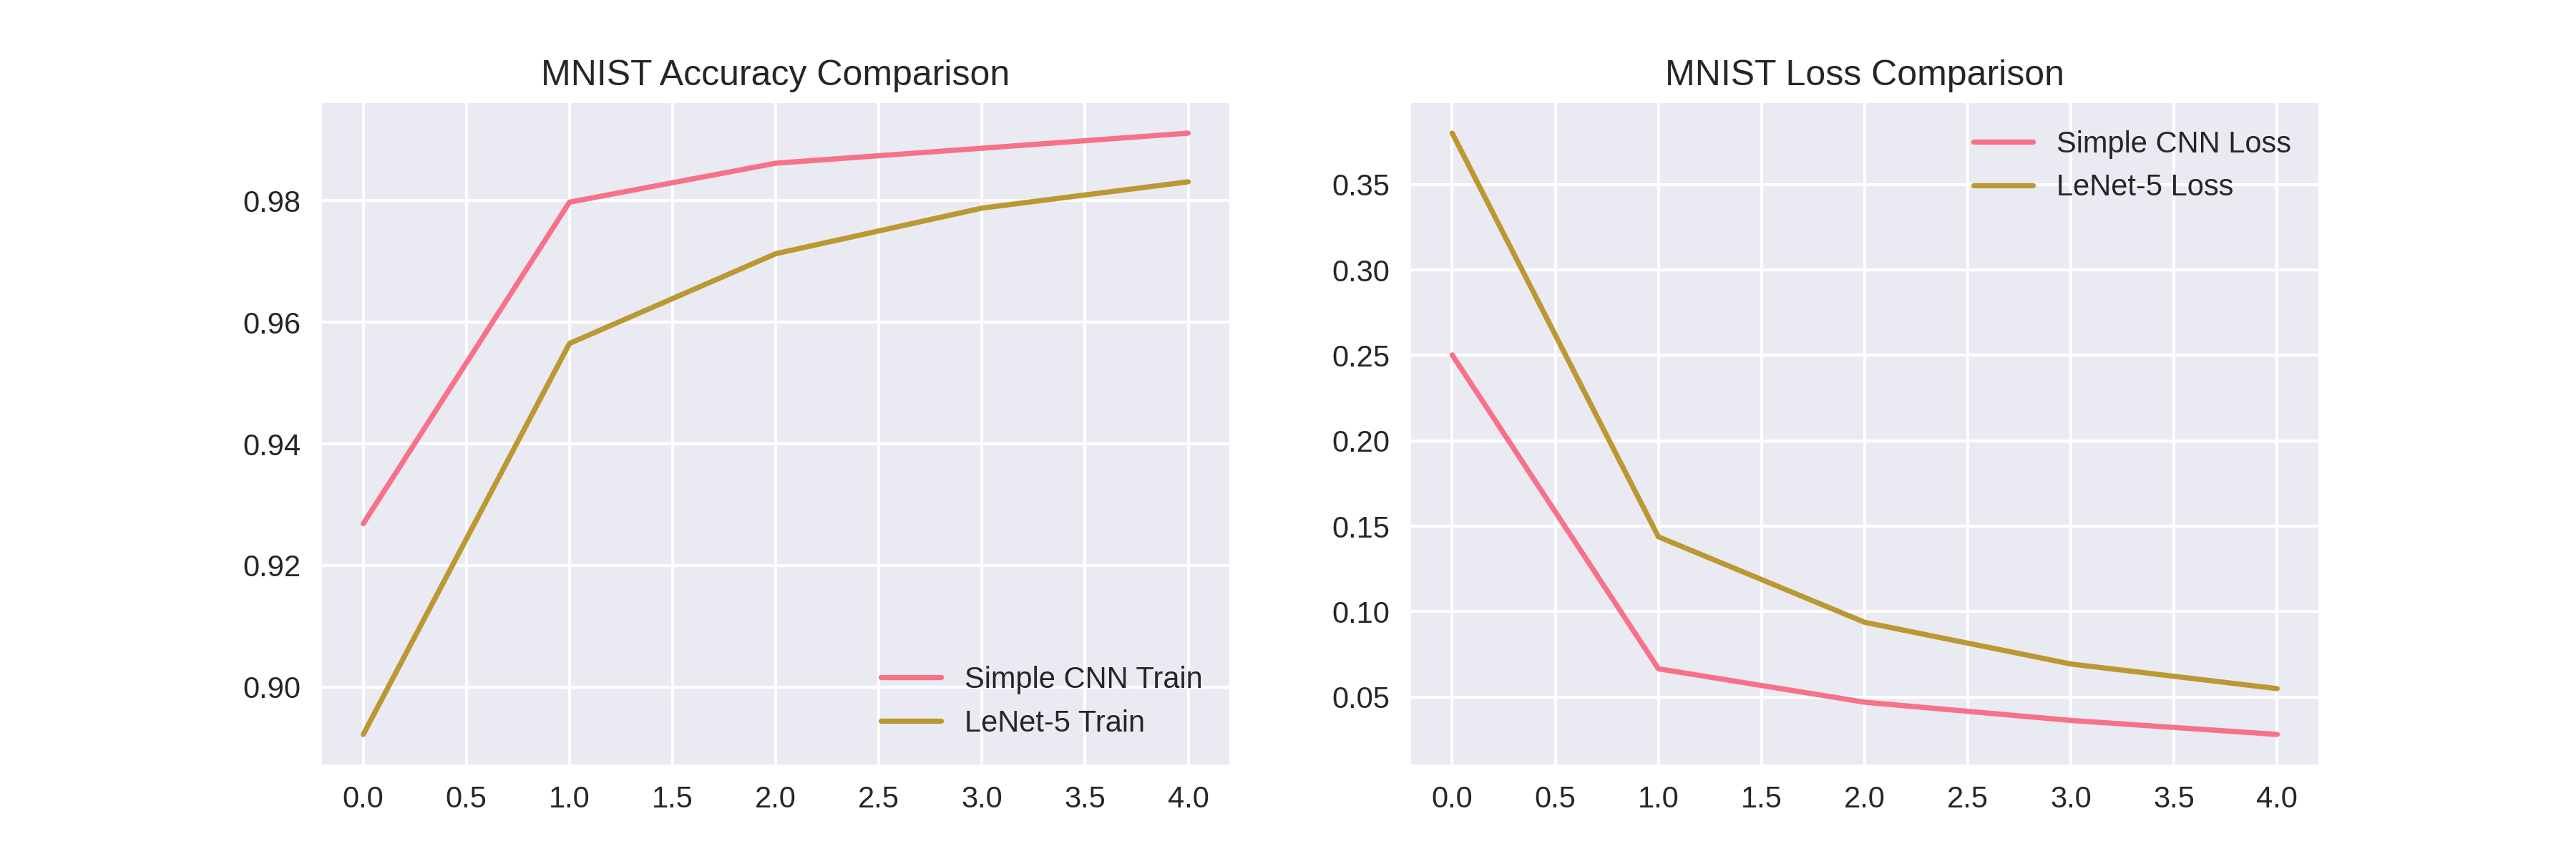
\includegraphics[width=0.75\textwidth]{../code/ch2_cnn/plots/ch2_mnist_history.png}
    \caption{So sánh lịch sử huấn luyện: Đồ thị cho thấy cả hai mô hình đều đạt độ chính xác trên 98\% chỉ sau vài epochs, tuy nhiên Simple CNN hội tụ nhanh hơn nhờ ReLU.}
\end{figure}

\begin{figure}[H]
    \centering
    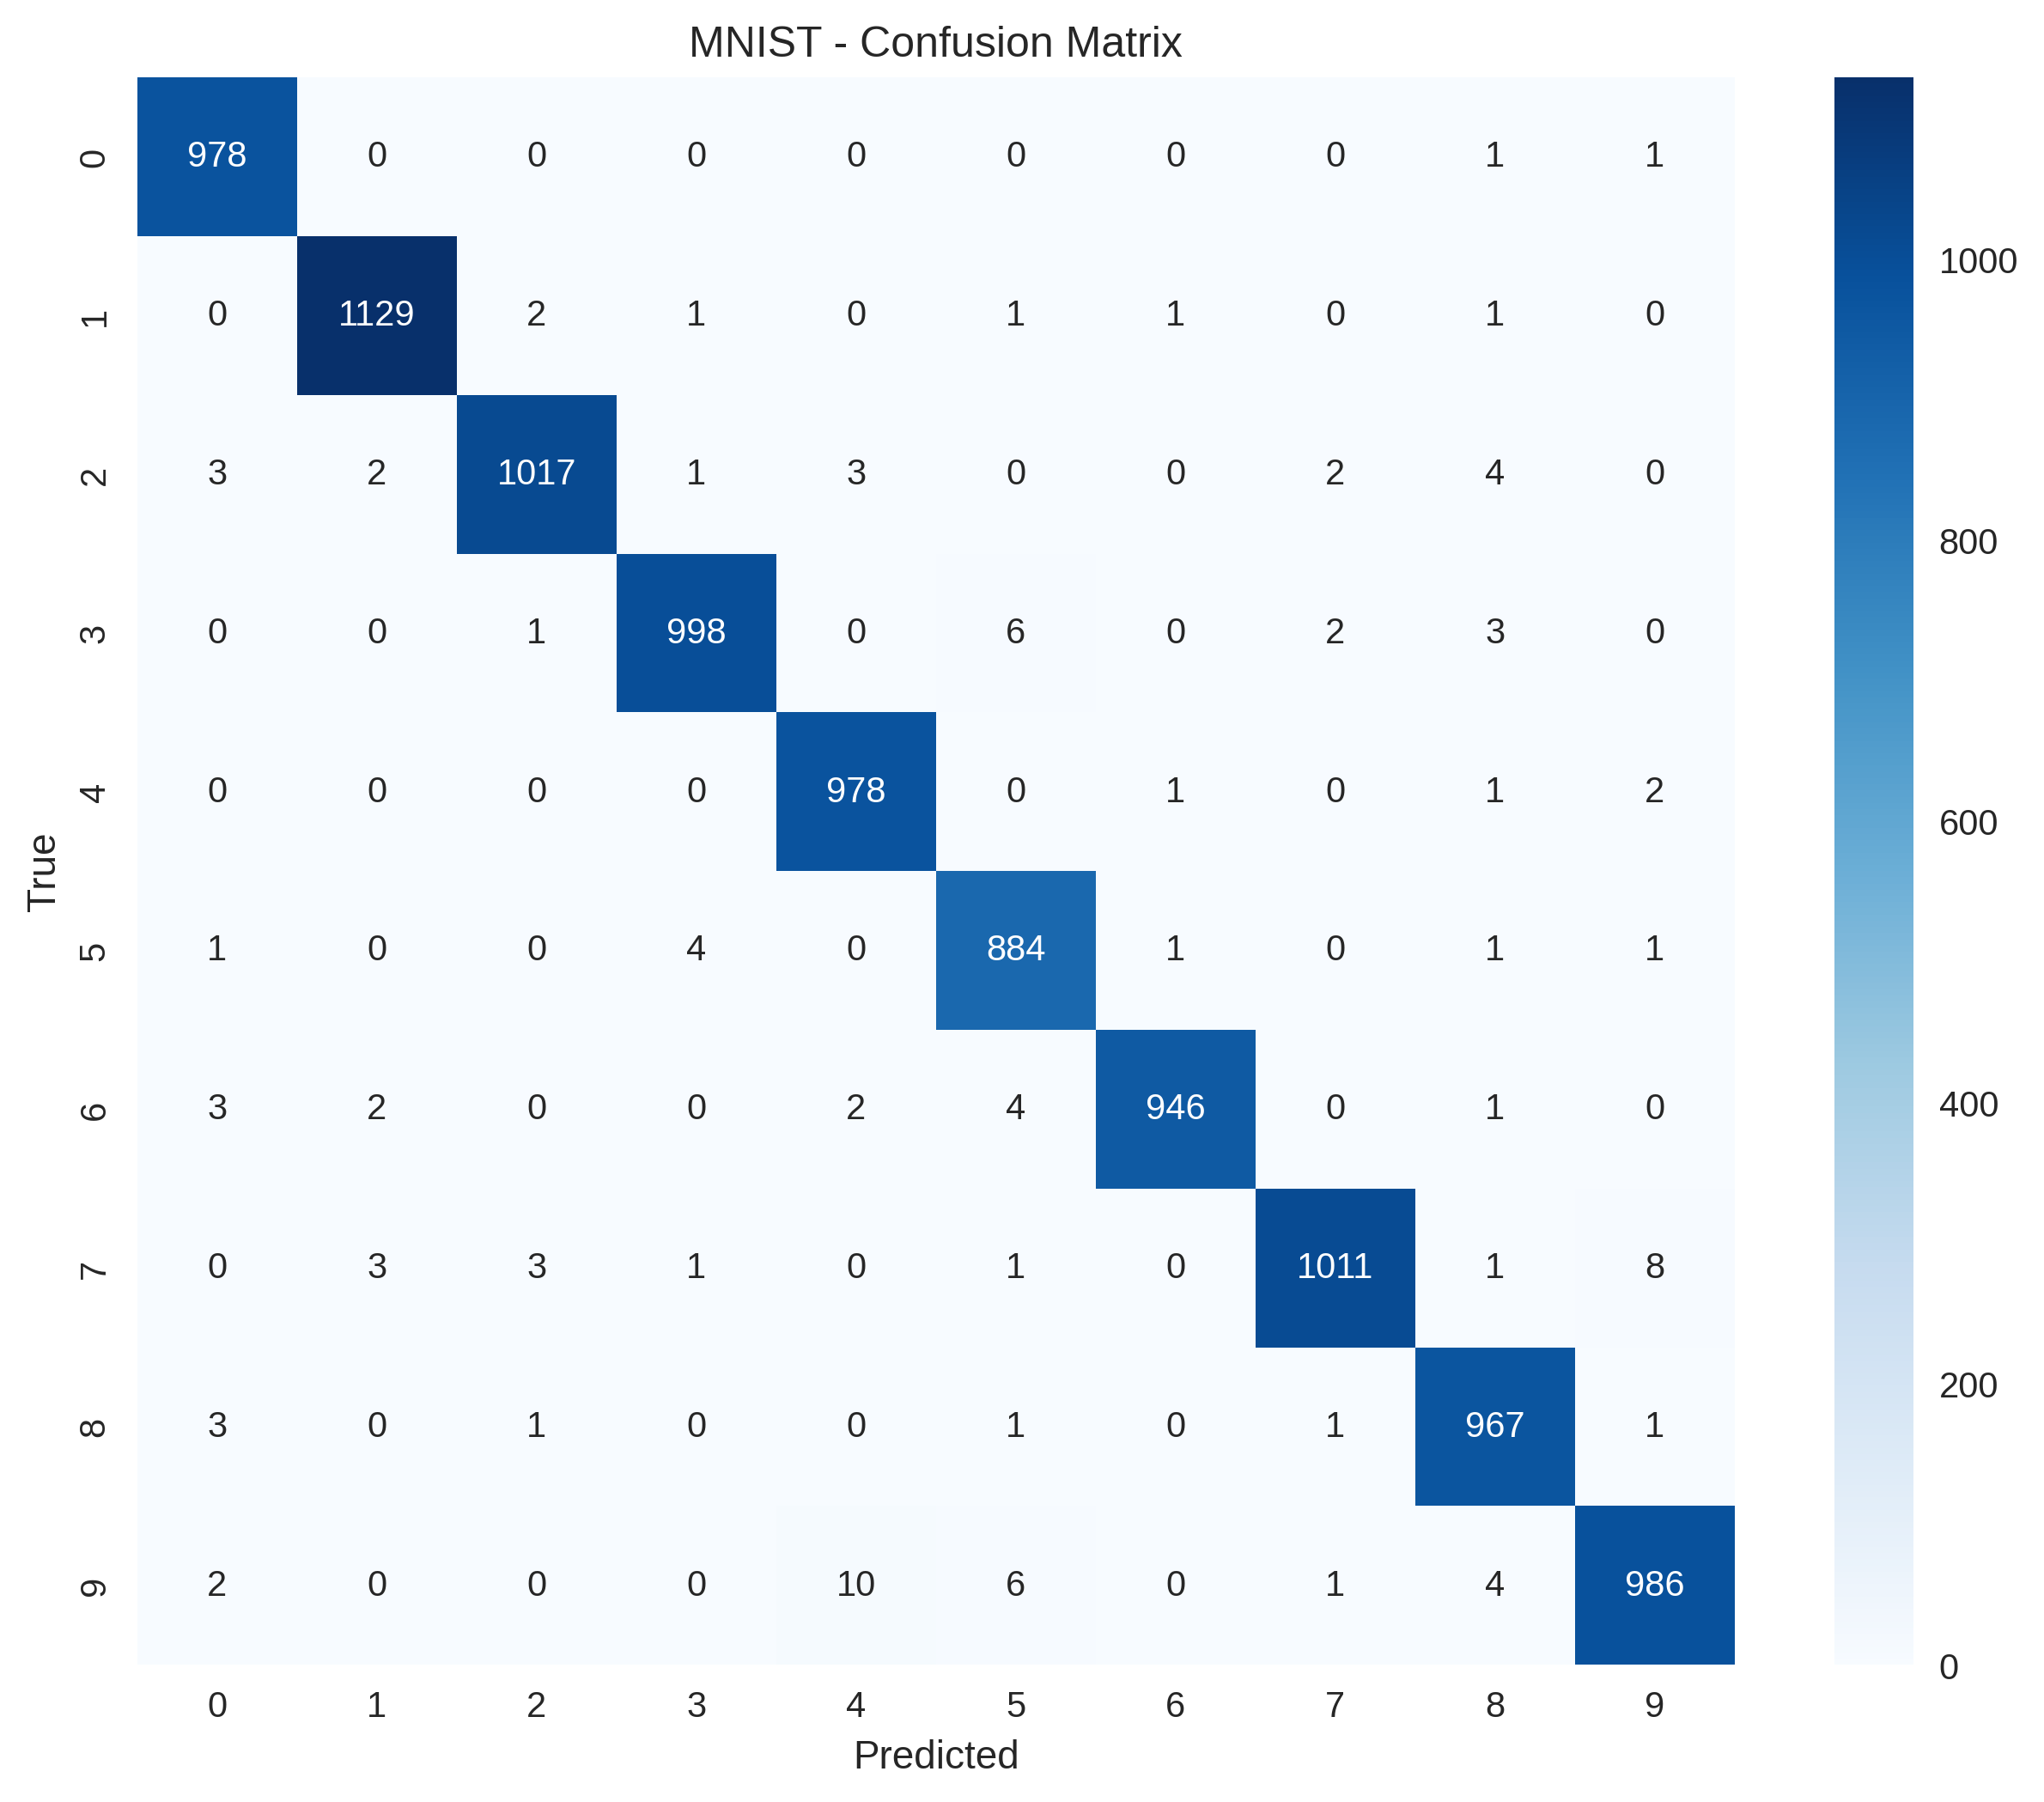
\includegraphics[width=0.75\textwidth]{../code/ch2_cnn/plots/mnist_confusion_matrix.png}
    \caption{Ma trận nhầm lẫn (Confusion Matrix): Phân tích chi tiết các cặp chữ số dễ gây nhầm lẫn (như 4 và 9, hoặc 3 và 5).}
\end{figure}

\begin{figure}[H]
    \centering
    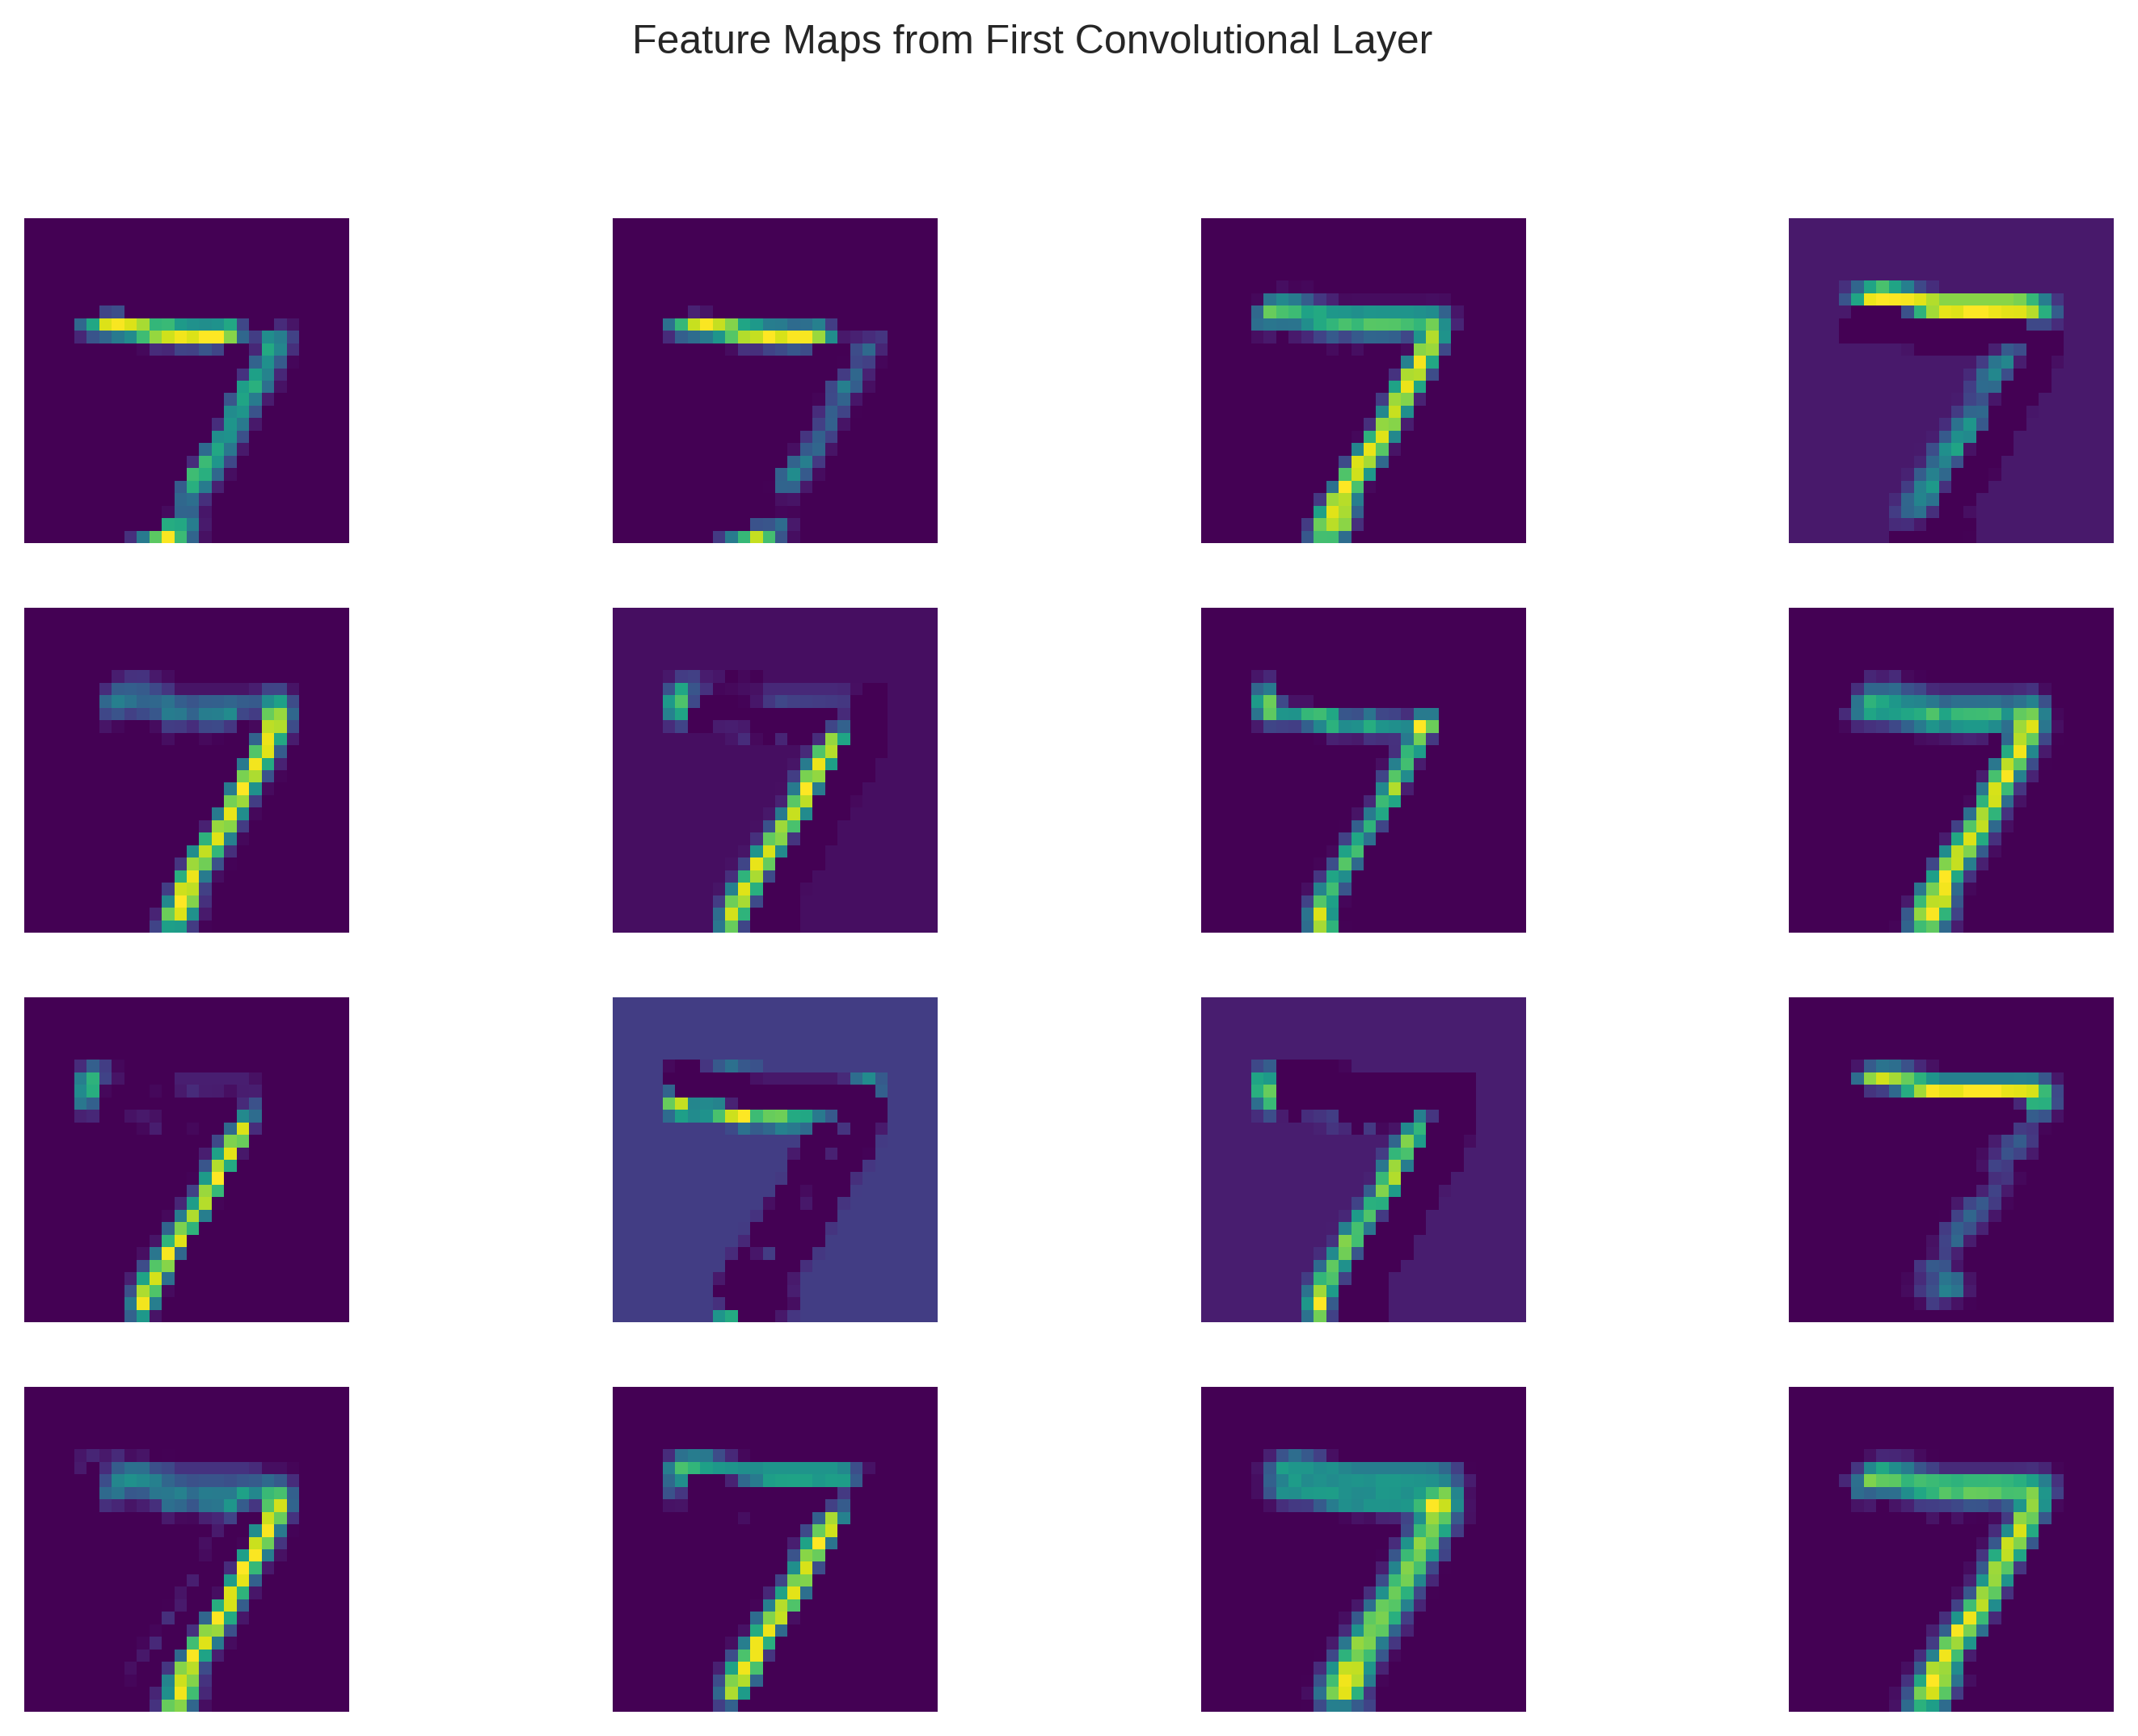
\includegraphics[width=0.75\textwidth]{../code/ch2_cnn/plots/mnist_feature_maps.png}
    \caption{Trực quan hóa Feature Maps: Hiển thị cách các bộ lọc (filters) ở lớp đầu tiên nhận diện các cạnh, góc và nét vẽ thô của chữ số.}
\end{figure}

\textbf{Kết nối thực nghiệm:} Quan sát các Feature Maps này, ta thấy lớp đầu tiên hoạt động tương tự như các toán tử phát hiện biên (như Sobel hay Canny) trong xử lý ảnh truyền thống. Tuy nhiên, thay vì được thiết kế tay, các bộ lọc này được CNN tự học thông qua quá trình lan truyền ngược (Backpropagation).

\subsubsection{Bài toán 2: Phân loại Fashion-MNIST}
Fashion-MNIST có độ phức tạp cao hơn do các mẫu ảnh trang phục chứa nhiều chi tiết tinh xảo hơn chữ số.

\begin{figure}[H]
    \centering
    
\includegraphics[width=0.9\textwidth]{../code/ch2_cnn/images/8.png}
    \caption{Nạp bộ dữ liệu Fashion-MNIST và chuẩn bị danh sách nhãn (class\_names) cho việc hiển thị.}
\end{figure}

\begin{figure}[H]
    \centering
    
\includegraphics[width=0.9\textwidth]{../code/ch2_cnn/images/9.png}
    \caption{Xây dựng hai phiên bản mô hình: Simple CNN và Deep CNN (có sử dụng BatchNormalization và Dropout để chống Overfitting).}
\end{figure}

\textbf{Vai trò của Regularization:} Trong mô hình Deep CNN, \texttt{BatchNormalization} giúp ổn định quá trình huấn luyện bằng cách chuẩn hóa đầu ra của mỗi lớp. Trong khi đó, \texttt{Dropout} ngẫu nhiên loại bỏ một tỷ lệ nơ-ron, buộc mạng không được phụ thuộc quá mức vào bất kỳ đặc trưng riêng lẻ nào, từ đó nâng cao khả năng tổng quát hóa (Generalization) trên dữ liệu chưa biết.

\begin{figure}[H]
    \centering
    
\includegraphics[width=0.9\textwidth]{../code/ch2_cnn/images/10.png}
    \caption{Mã nguồn so sánh hiệu suất giữa mạng CNN đơn giản và mạng CNN sâu trên bộ dữ liệu trang phục.}
\end{figure}

\begin{figure}[H]
    \centering
    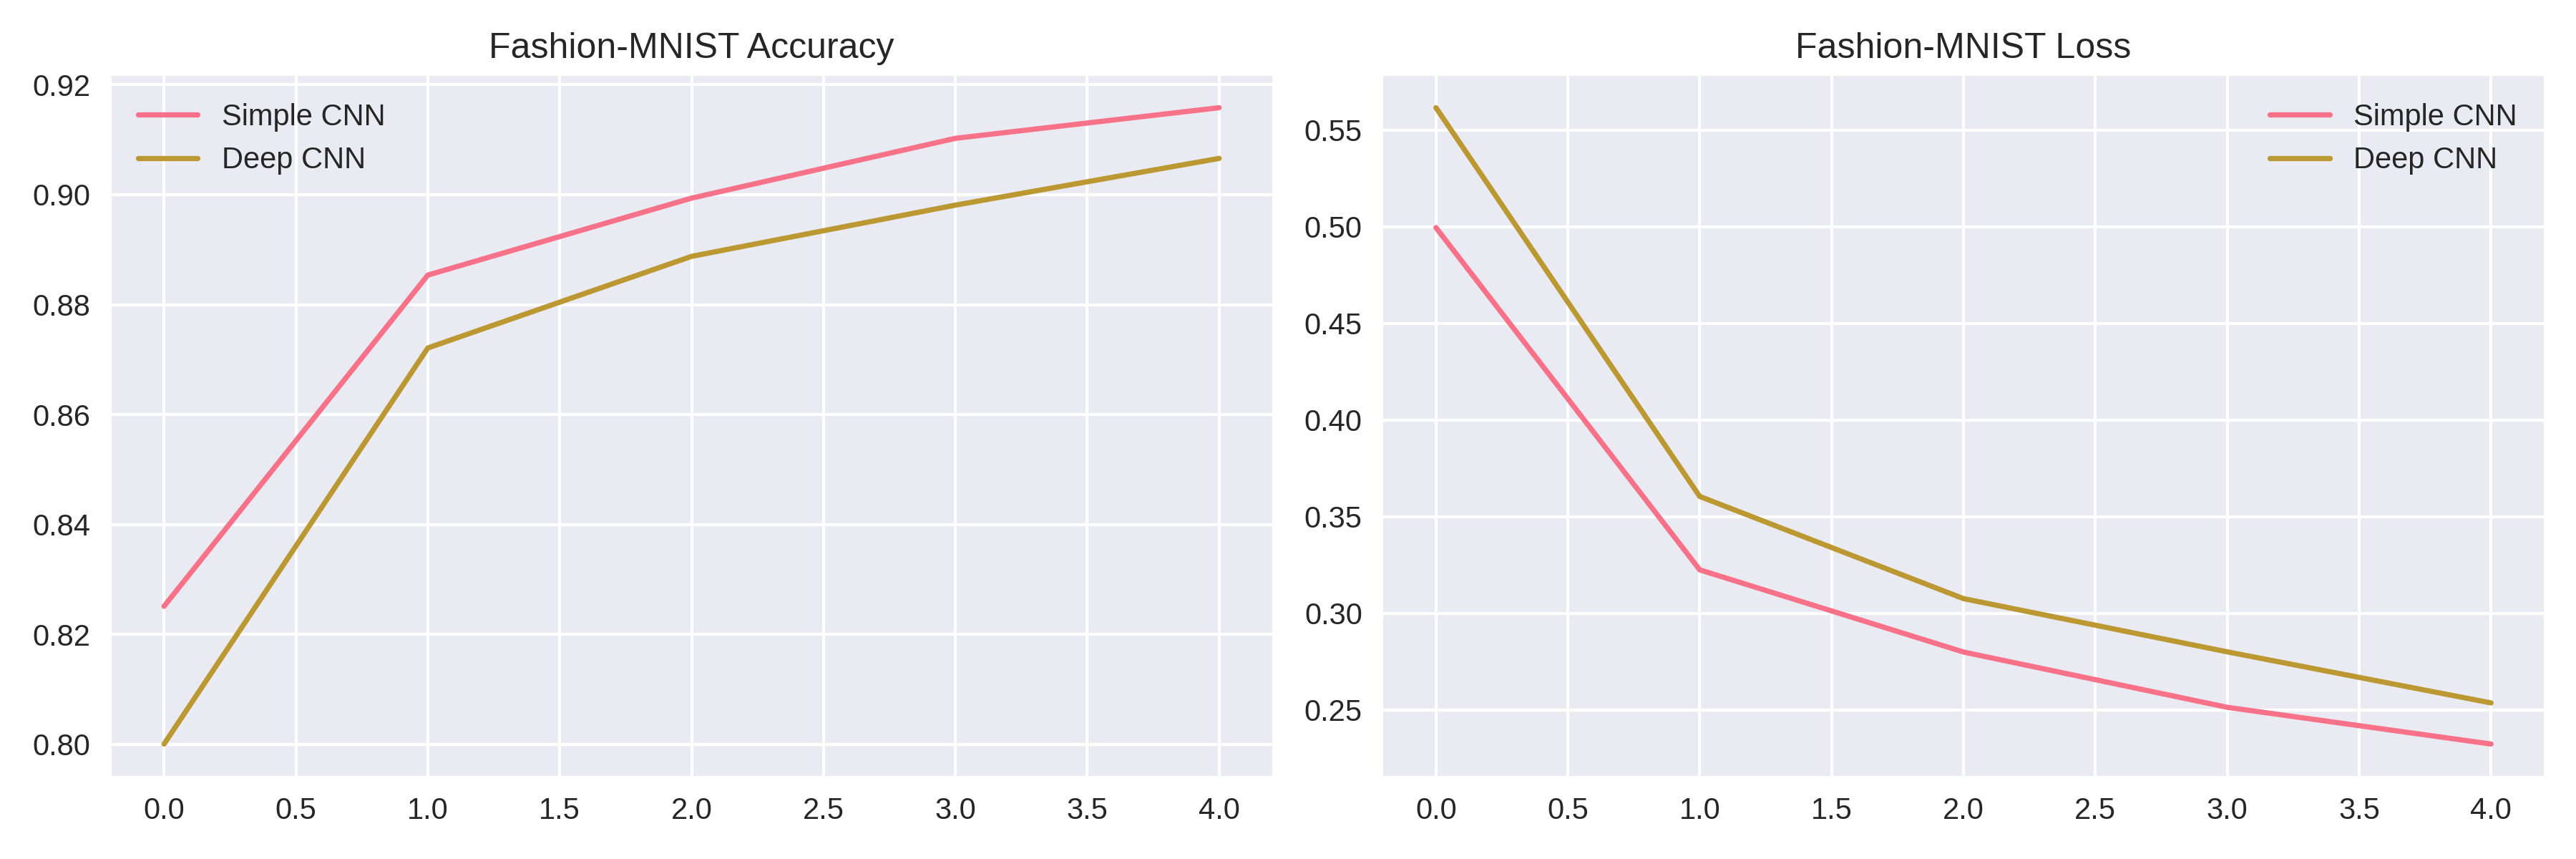
\includegraphics[width=0.75\textwidth]{../code/ch2_cnn/plots/ch2_fashion_history.png}
    \caption{So sánh hội tụ: Deep CNN đạt kết quả ổn định hơn nhờ các lớp Regularization, mặc dù thời gian huấn luyện mỗi epoch lâu hơn.}
\end{figure}

\begin{figure}[H]
    \centering
    
\includegraphics[width=0.9\textwidth]{../code/ch2_cnn/images/11.png}
    \caption{Mã nguồn thực hiện EDA chi tiết cho Fashion-MNIST để phân tích tính đa dạng của các loại trang phục.}
\end{figure}

Các kết quả phân tích Fashion-MNIST:

\begin{figure}[H]
    \centering
    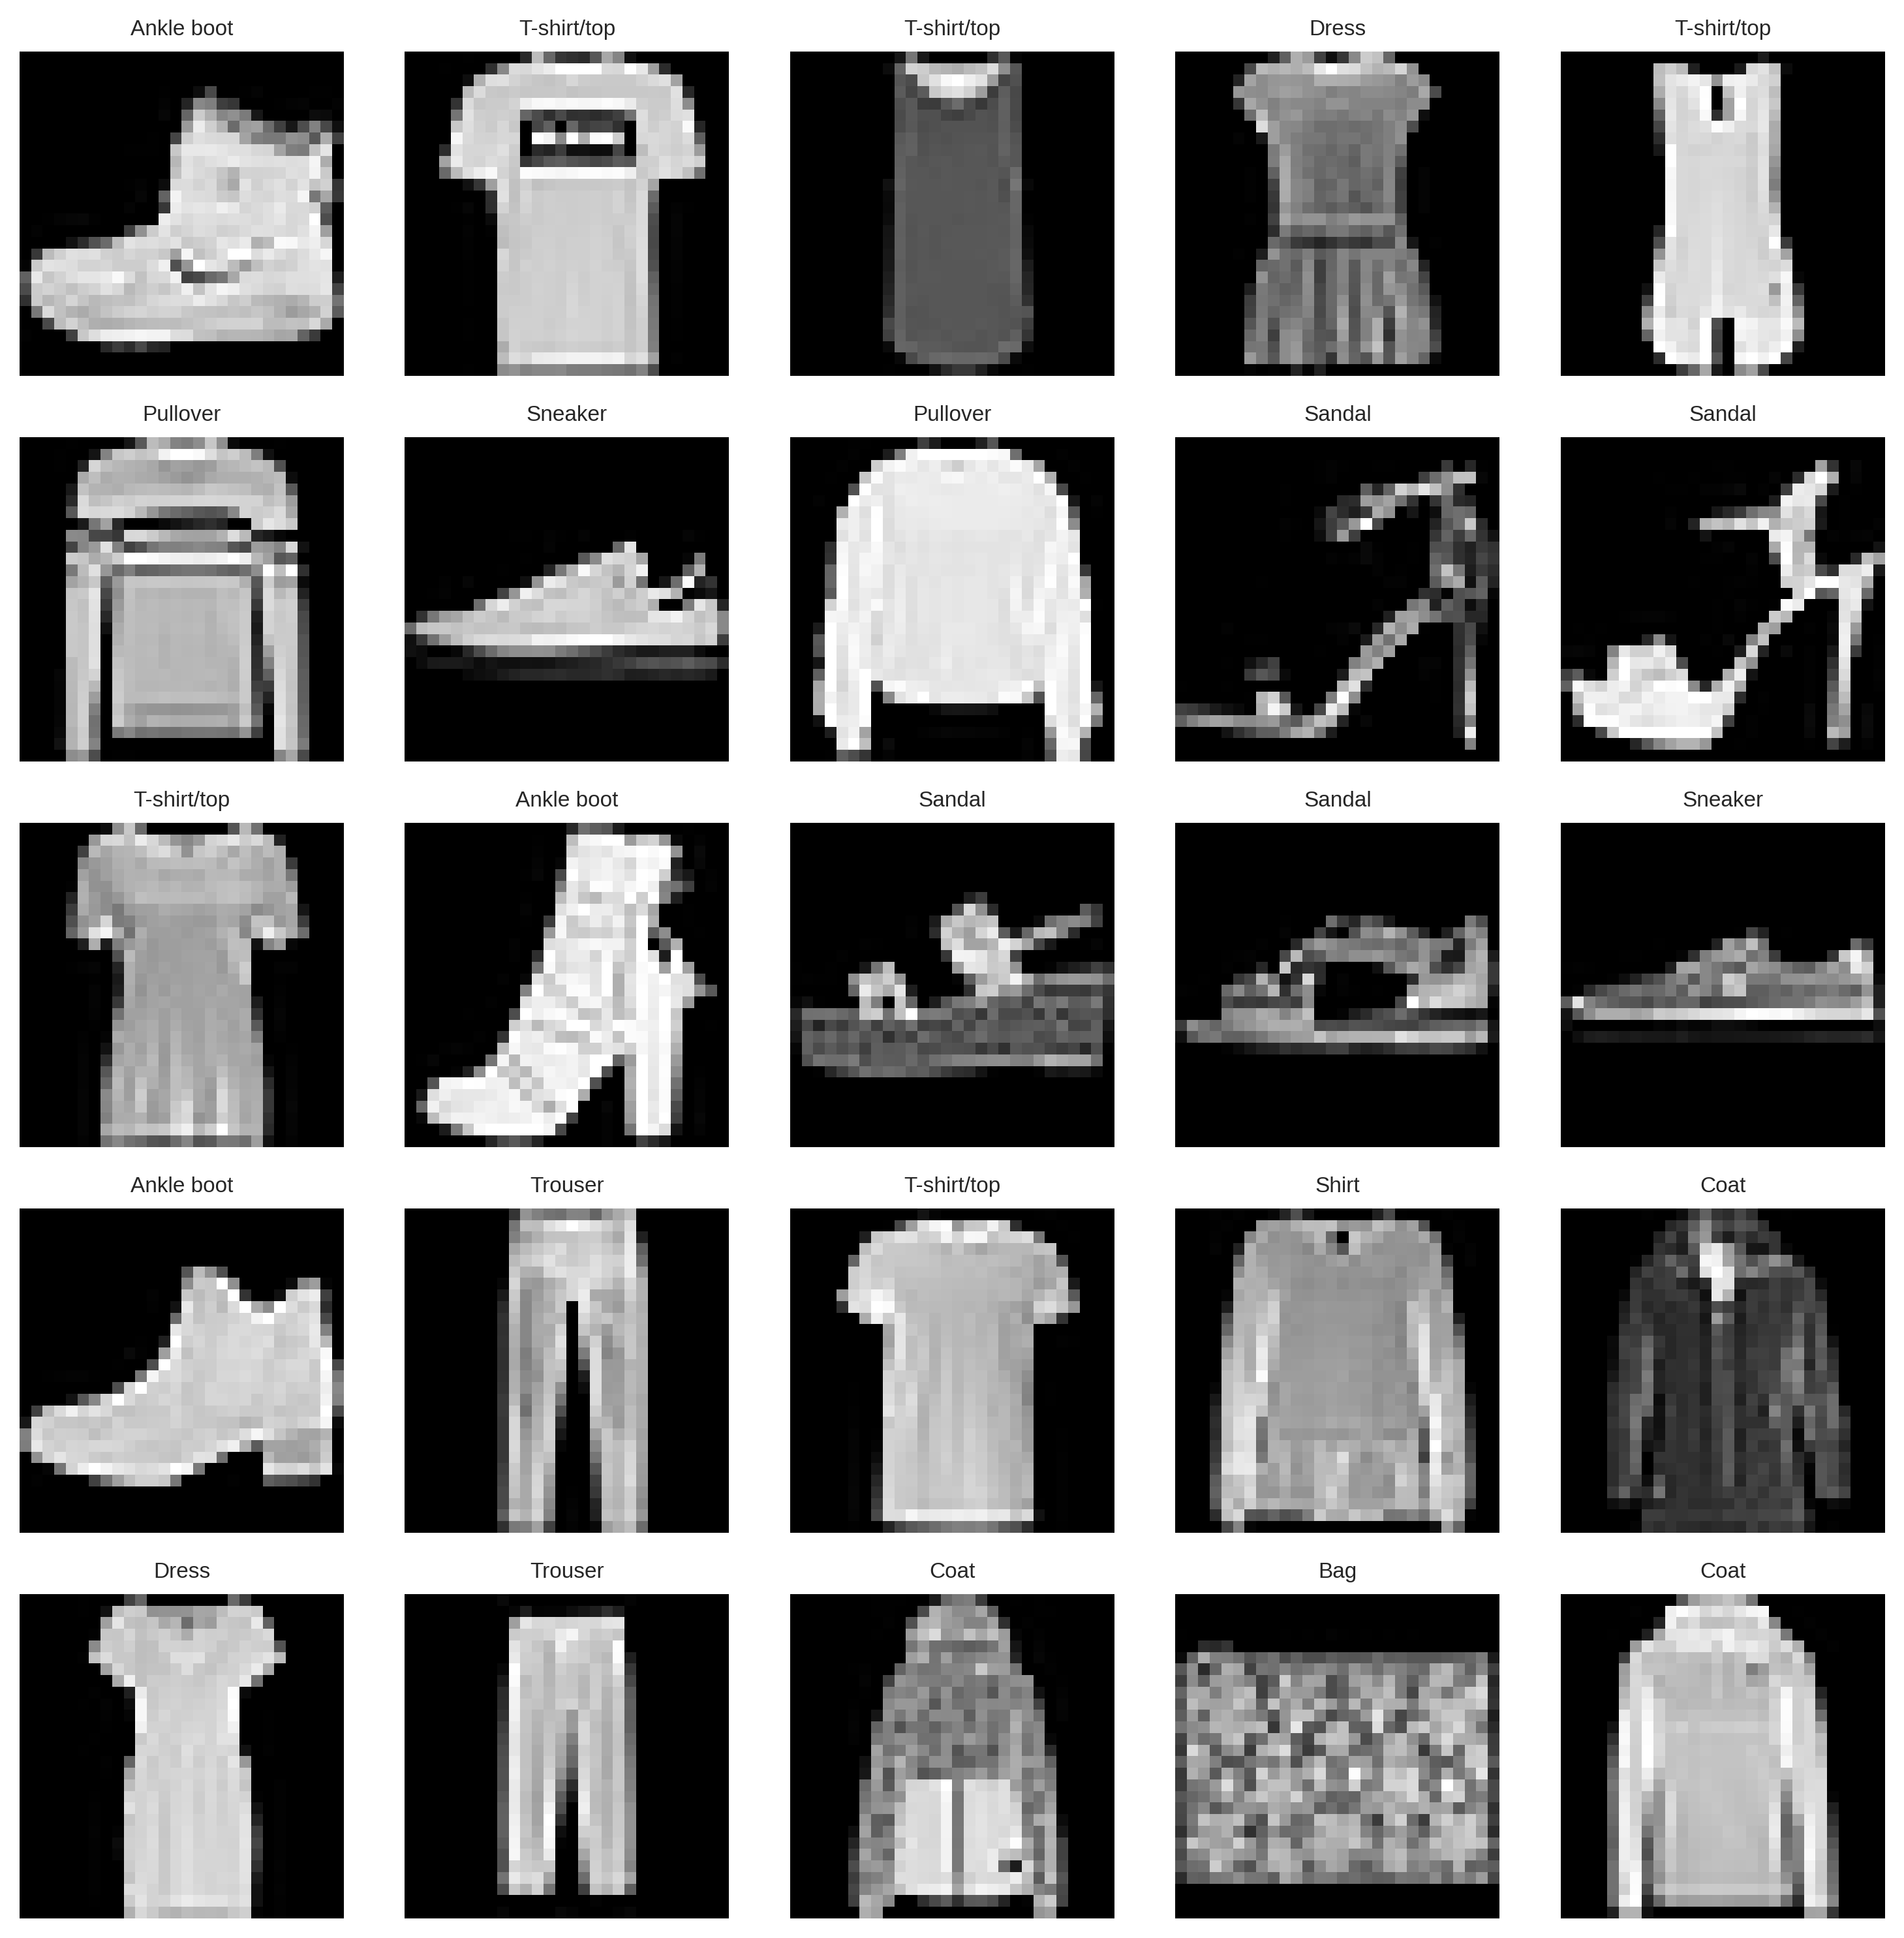
\includegraphics[width=0.75\textwidth]{../code/ch2_cnn/plots/fashion_mnist_sample_images.png}
    \caption{Mẫu trang phục: Hiển thị 25 sản phẩm thời trang đại diện cho 10 lớp nhãn khác nhau.}
\end{figure}

\begin{figure}[H]
    \centering
    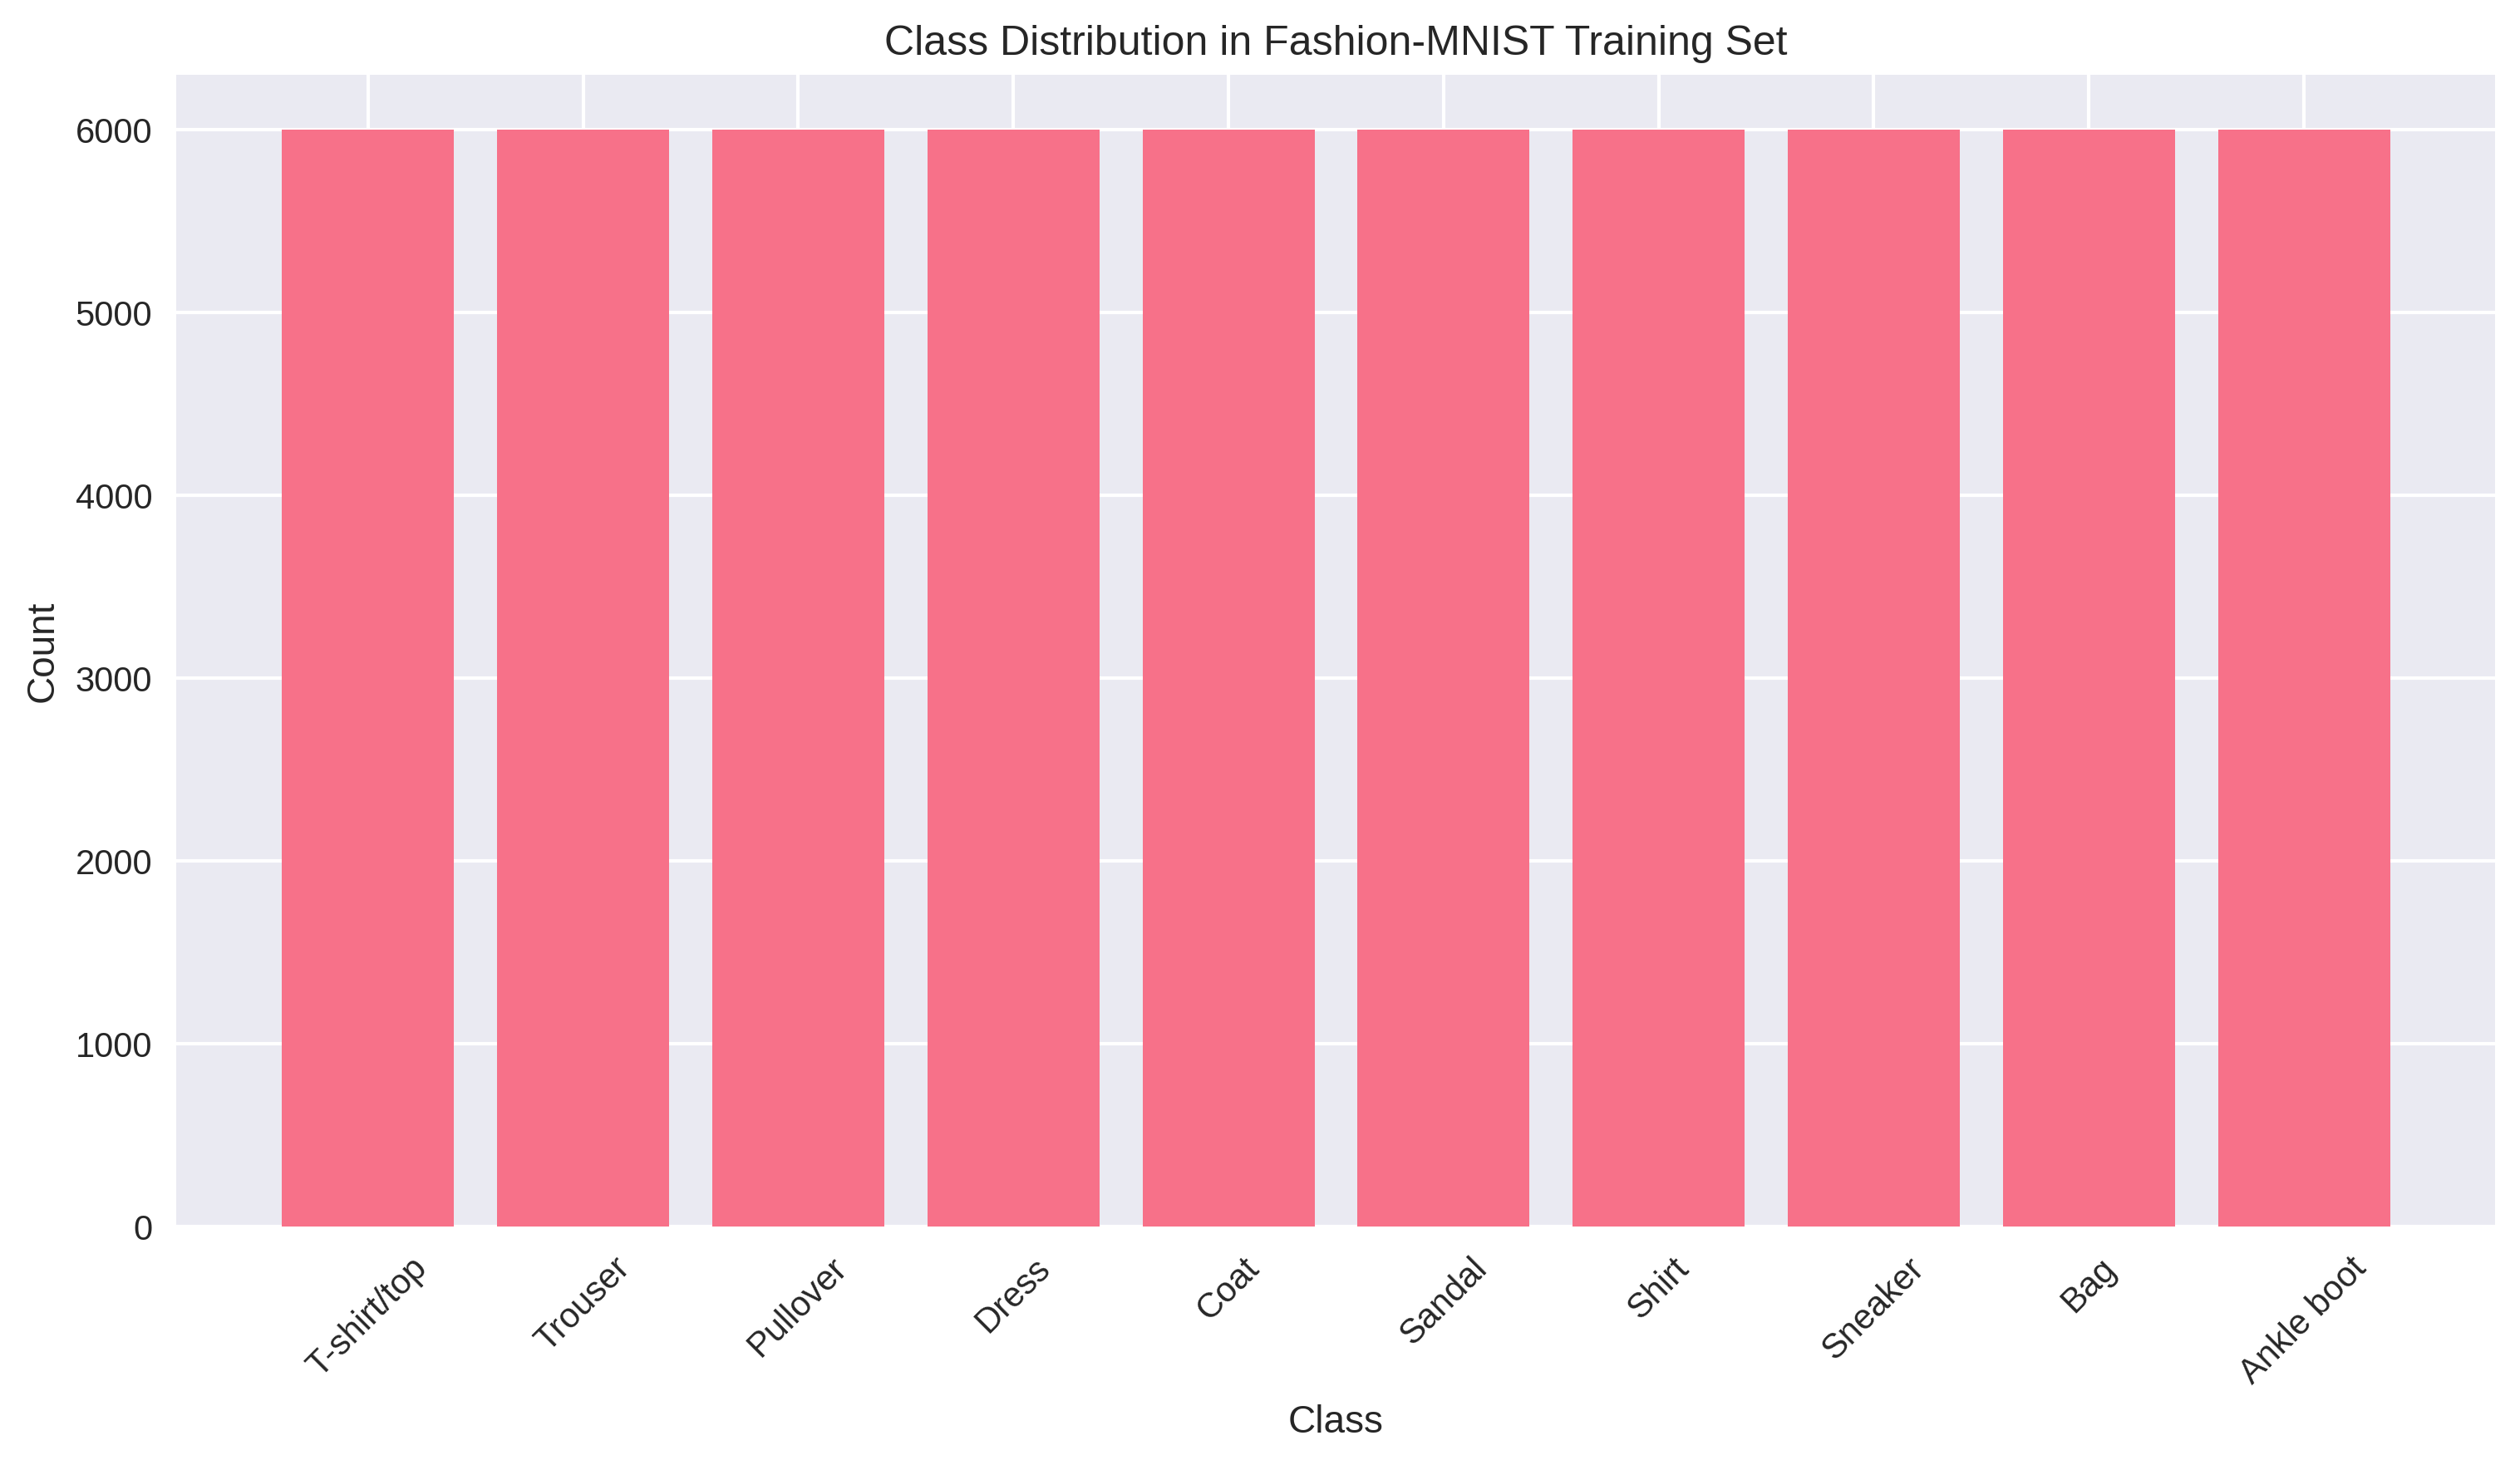
\includegraphics[width=0.75\textwidth]{../code/ch2_cnn/plots/fashion_mnist_class_distribution.png}
    \caption{Sự cân bằng dữ liệu: Khẳng định tính chuẩn mực của bộ dữ liệu Fashion-MNIST với số lượng mẫu đồng đều cho mọi loại trang phục.}
\end{figure}

\begin{figure}[H]
    \centering
    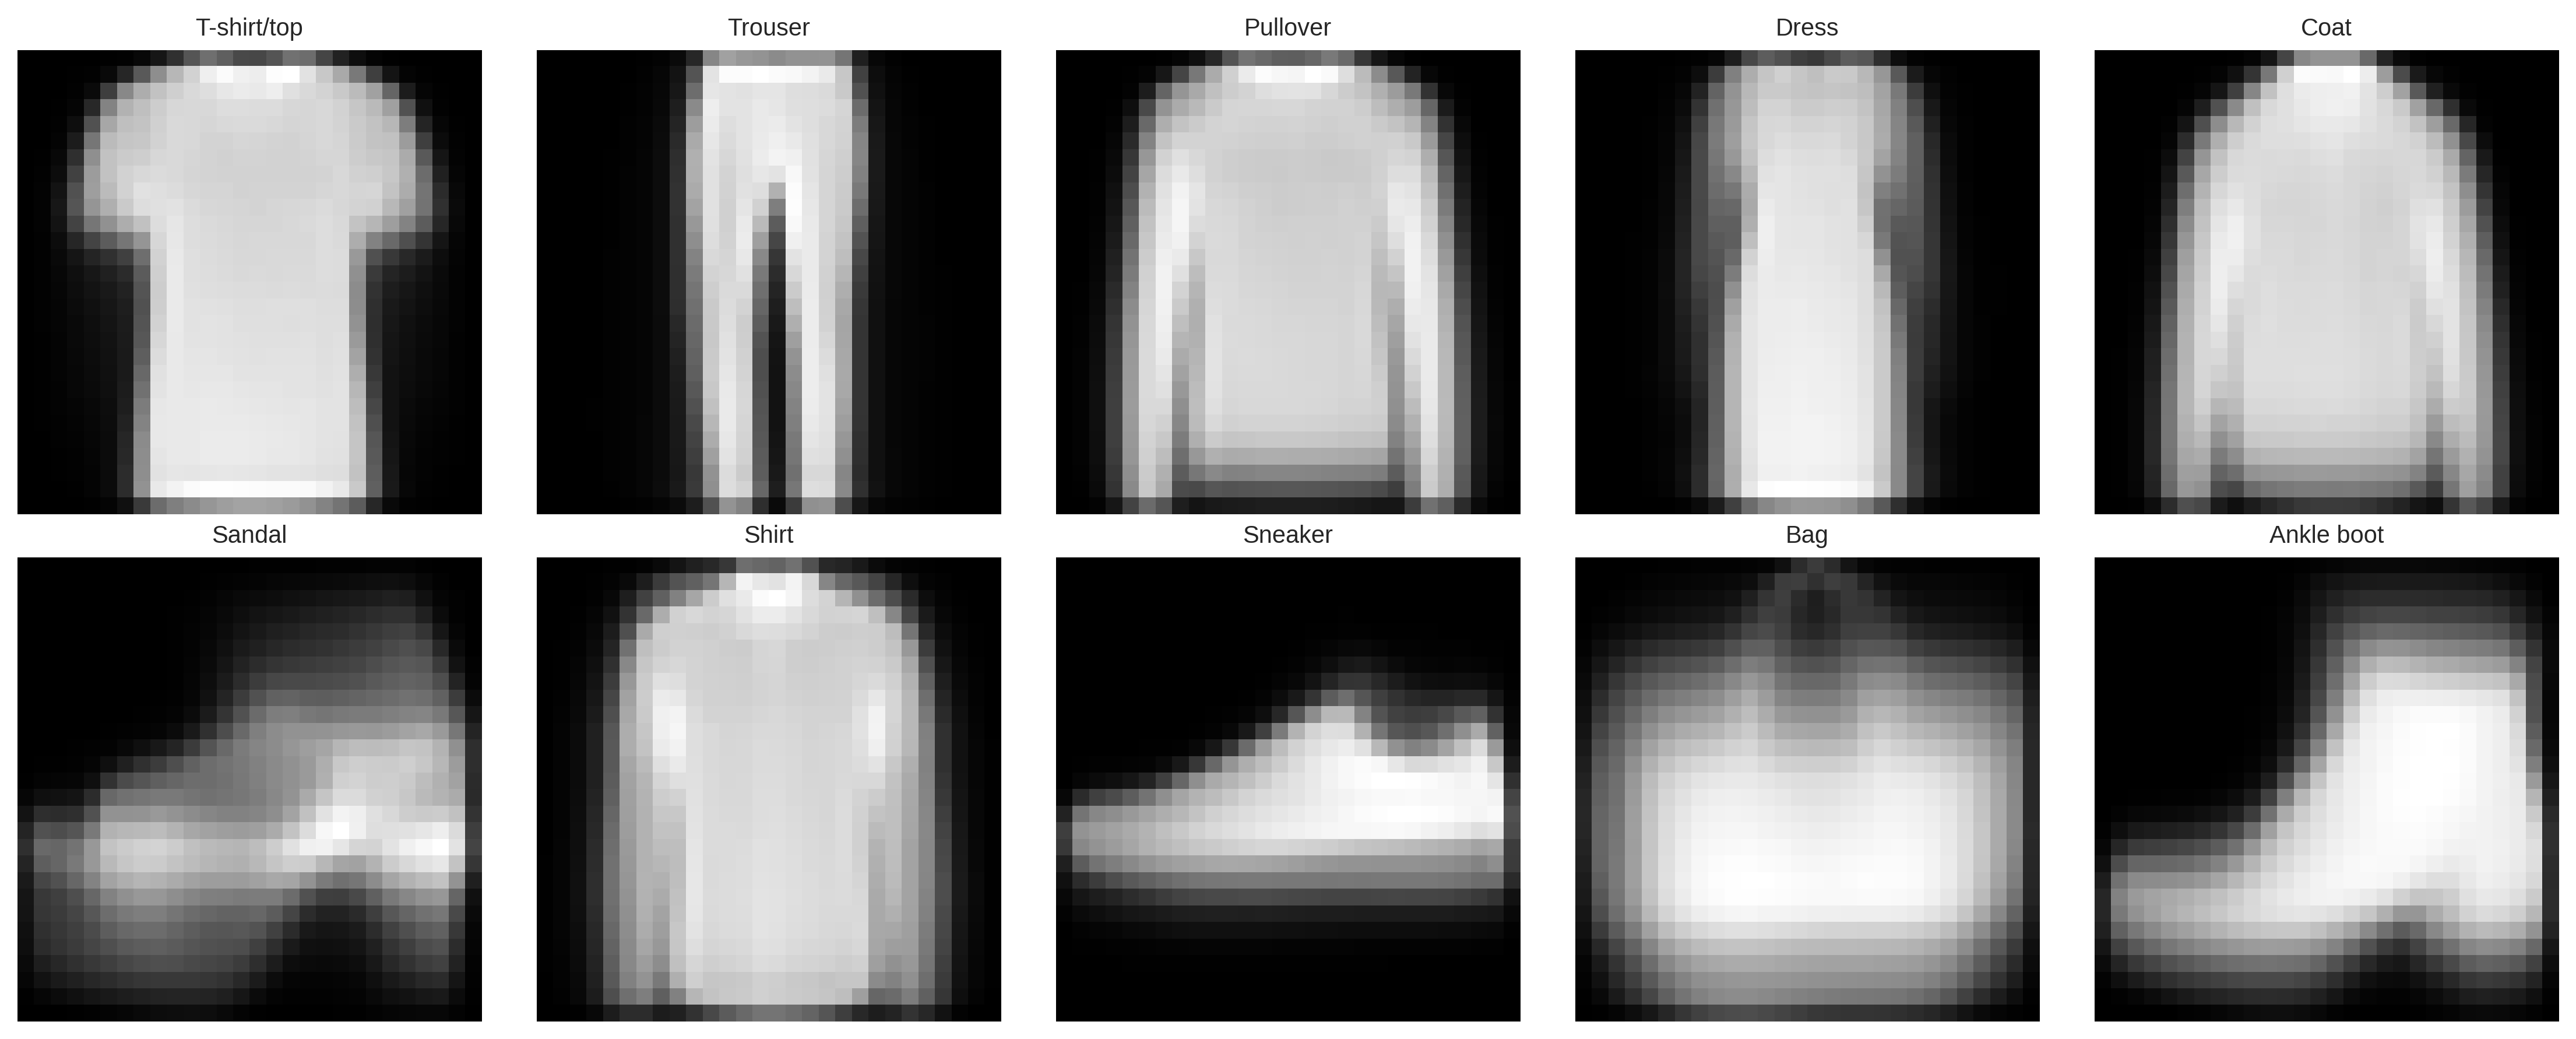
\includegraphics[width=0.75\textwidth]{../code/ch2_cnn/plots/fashion_mnist_average_items.png}
    \caption{Hình dáng trung bình của trang phục: Giúp nhận diện các đặc điểm chung của từng lớp (ví dụ: tay áo dài của Coat so với T-shirt).}
\end{figure}

\begin{figure}[H]
    \centering
    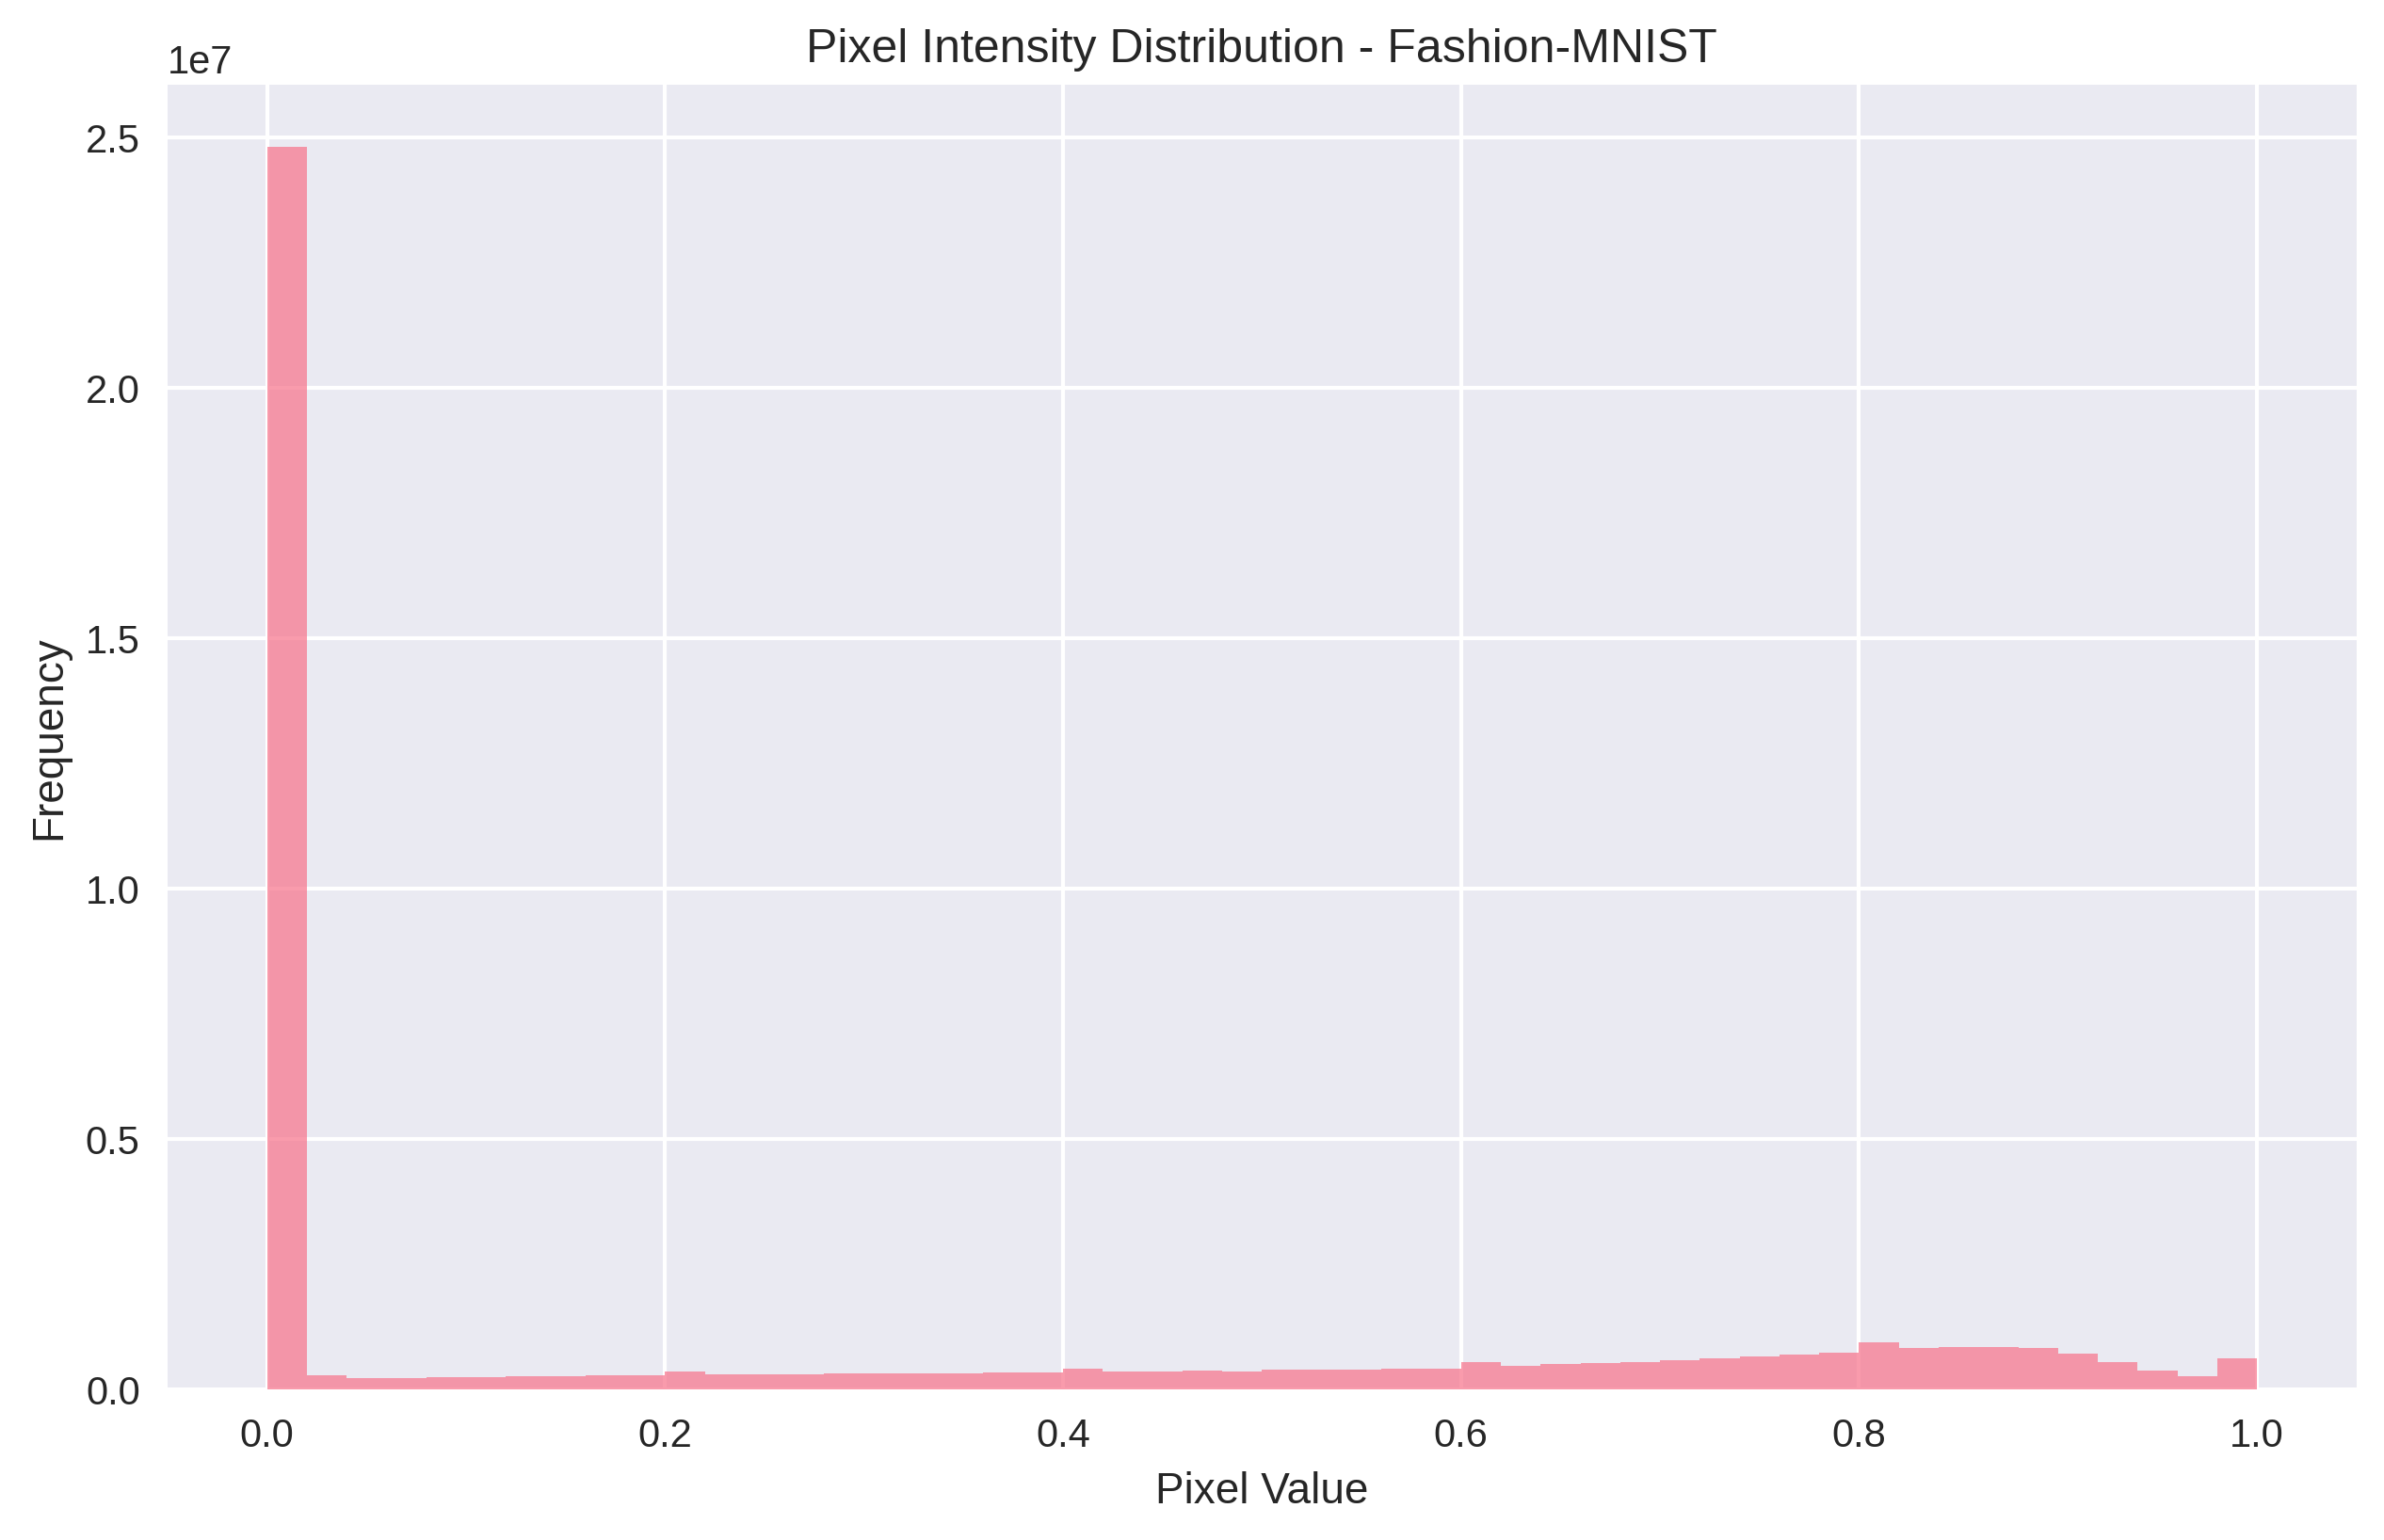
\includegraphics[width=0.75\textwidth]{../code/ch2_cnn/plots/fashion_mnist_pixel_intensity_distribution.png}
    \caption{Phân phối cường độ Pixel: Phản ánh độ phức tạp cao hơn của ảnh trang phục so với ảnh chữ số (nhiều mức xám trung gian hơn).}
\end{figure}

\subsection{Kết luận Chương 2}
Thông qua các thực nghiệm trên MNIST và Fashion-MNIST, chúng ta đã chứng minh được sức mạnh trích xuất đặc trưng của mạng CNN. Việc tinh chỉnh kiến trúc (như thêm Dropout, BatchNormalization) và lựa chọn hàm kích hoạt phù hợp (ReLU) đóng vai trò then chốt trong việc cải thiện hiệu suất mô hình.

Đặc biệt, việc trực quan hóa Feature Maps và Confusion Matrix đã giúp chúng ta có cái nhìn sâu sắc hơn về cách mạng nơ-ron "nhìn" và "phân loại" hình ảnh.